\chapter{ASR --- Automatic Speech Recognition}\label{ch:asr_ch}
\section{Introduction}
Speech recognition (SR) stands for recognizing 
natural speech and translating 
it to readable text named transcript.
Often speech recognition is referred to as Speech-to-Text (STT). 
Speech recognition 
that is accomplished 
automatically by a computing machine or 
software is known as ASR (Automatic Speech Recognition).

ASR systems employ numerous algorithms 
and techniques to conduct the speech to text translation.
Some algorithms aim for precision improvements
and higher detection ratios measured with \emph{WER},
\emph{CER}
and \emph{PER},
as described in Chapter\;\ref{ch:features}.
Other algorithms target increasing to increase
the system's robustness, which means
how well the system can still function adequately
given that the environmental conditions
are not static and change.

Naturally spoken speech has inherent 
variabilities depending on many 
factors that make a speech signal 
classified as non-stationary and inconsistent. 
Natural speech heavily depends on the speaker's gender, 
whether a male or a female and the speaker's age. 
Moreover, different speakers of the same 
gender and age range may still present variances 
in the vocal range, pitch, and formant frequencies.
Likewise, we can say that Gender-independent 
characteristics such as accent, style of speech, emotional state, 
or health conditions, 
which are examples of social and geographical factors, 
all impact naturally spoken sentences and 
introduce some degree of variability.

Due to the high dependency that natural speech has on so many factors, 
an ASR system must have high endurance to fluctuations in these 
previously mentioned artifacts. Also, the ability to perform adequately in a wide range of scenarios is very crucial.  
In particular, the cases of high background noise levels in low SNR scenarios and multiple reverberations due to poor room acoustics.

Traditional ASR engines 
are usually built of several sets, 
where each set contains a module or several 
modules designated for a specific task.
An ASR engine as a whole is a chain of these modules connected in a pipeline. 
A common structure of an ASR system
is shown in Figure\;\ref{fig:asr_blocks}. This type
of ASR system translates a speech waveform into a transcript
by chaining \emph{phonemes} together to construct words.

A phoneme is a discrete and distinctive unit of language
that can be used to differentiate between words.
A word is a sequence of phonemes chained together in how the word is 
actually pronounced. 
The motivation of detecting phonemes instead of entire words by the ASR engine relies on the fact that the number of words in a common language crosses the tens of thousands and sometimes even larger than hundreds of thousands. 
Extensive word vocabulary implies a huge training dataset 
requirement covering most of the words in a selected language.
On the contrary, most languages have 20-60 phonemes\cite{Blust2013TerrorFT, dixon_1997}.
In that way, a much smaller set of dedicated phonemes can be used to construct the vocabulary utilizing a less demanding training dataset requirement.

\begin{figure}[H]
    \centering
    \subfloat[\label{fig:asr_blocks}]{%
       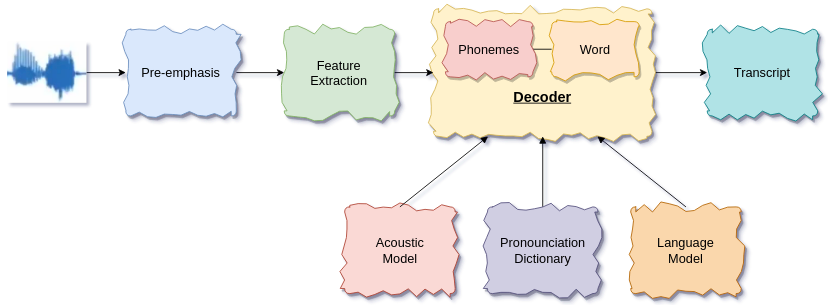
\includegraphics[width=0.75\linewidth]{ASR/images/asr_blocks}}
    \\
    \subfloat[\label{fig:e2e_asr_blocks}]{%
        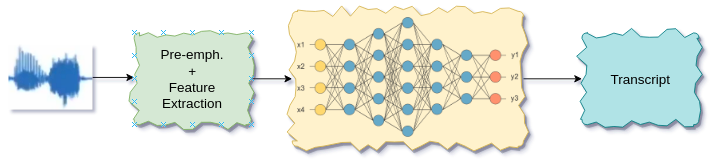
\includegraphics[width=0.75\linewidth]{ASR/images/e2e_asr_blocks}}
    \caption{(a) Traditional ASR system blocks diagram;\;\;
        (b) End-to-end ASR system blocks diagram.}\label{fig:tr_e2e_asr_blocks} 
\end{figure}

The system presented in Figure\;\ref{fig:asr_blocks} 
shows a pipeline that starts with a pre-emphasis and features
extraction modules. 
The pre-emphasis accounts for the speech analysis, noise cancellation, speech enhancements, windowing, and framing of the speech into sub-frames in which it is closer in characteristics to a stationary signal.
The feature extraction module extracts the individual features representing the speech from the incoming frames as MFCCs, FilterBanks, and others.

The next module in line is the decoder. The decoder's responsibility is to take the features, convert them to a set of phonemes and chain them together to detectable words, composing the transcript at the output.
A decoder is built from three sub-models tied
together that work in harmony. 
The first is the Acoustic Model (AM), which maps the acoustic features extracted in the earlier module to phoneme sequences with probabilistic weights.
These phonemes are an intermediate representation in the process of word decoding.
An additional module is the pronunciation model. This module is a dictionary, handcrafted by an expert linguist and tailor-made to each language explicitly.
This dictionary links phoneme sequences
to words. 
Lastly, the Language Model (LM) calculates the likelihood a given word is detected based on the perceived phoneme sequences and how likely it is for this word to occur given the past temporal context.
The words or N-Grams with the highest scores are selected and written into the output transcript.

A newer more modernized approach known as 
End-to-End Automatic Speech
Recognition (E2E ASR) has been proposed 
in \cite{pmlr-v32-graves14}. This approach 
replaces the conventional decoder structure with 
a deep neural network of some kind that maps 
acoustic features to characters. An E2E ASR system
structure is presented in Figure\;\ref{fig:e2e_asr_blocks}.

With this architecture, there is no longer a need for expert 
dictionaries or complex models of chaining phonemes to words.
That spares the need to acquire new pronunciation models or maintain an existing one, which can be expensive. 
Instead, character probabilities 
are given at the output according to the learning
process of mapping acoustic features to 
corresponding letters.
That leads to another advantage of E2E ASR systems
over traditional ASRs. 
Retraining an E2E model with 
a new dataset of annotated speech in different 
languages is possible without changing the architecture at all.
On the other hand, 
using E2E systems means a more extensive training dataset is 
required for the model to generalize well, 
only to maintain comparable detection 
ratios in terms of WER and CER as the traditional ASRs do.

However, despite having an E2E system trained against a huge dataset, the direct estimations of characters and, later on, the construction of a full 
transcript don't work as expected compared to traditional ASRs.
To overcome the degradation in performance, several algorithms
can be applied to improve different aspects of the model.
Such a helpful technique that is 
called CTC (Connectionist Temporal Classification) 
by Maas et al. is presented \cite{maas-etal-2015-lexicon}.
This method demonstrates which characters get the highest 
probability for specific phonemes, 
as shown in
Figure\;\ref{fig:CTC_maas_graph}. 
Therefore, a more accurate selection of 
letters is achievable by utilizing a \emph{beam-search}.

\begin{figure}[H]
    \centering
    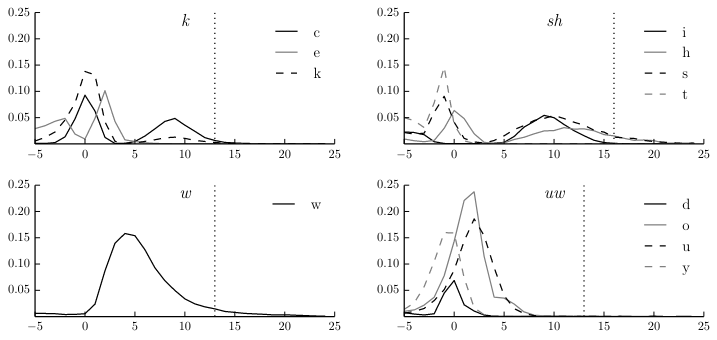
\includegraphics[width=0.95\linewidth]{ASR/images/CTC_maas_graph}
    \caption{Maas et al. \cite{maas-etal-2015-lexicon} phonemes vs characters graphs}\label{fig:CTC_maas_graph}
\end{figure}

Additional paradigm by Chan et al. known as Seq2Seq (Sequence-to-Sequence) or sometimes as Attention Encoder-Decoder (AED) networks
is presented in \cite{44926}.
 more known as
This approach is based on an LSTM transducer.
A more advanced model that is known for its self-attention mechanism 
was later suggested by Vasawani et al. in 2017 \cite{vaswani2017attention}.
This model, which also uses the Encoder-Decoder architecture, is called a transformer.

A sophisticated combination of these techniques is practically used in this work to construct and evaluate the different tested ASR engines.

% \begin{figure}[H]
%     \centering
%     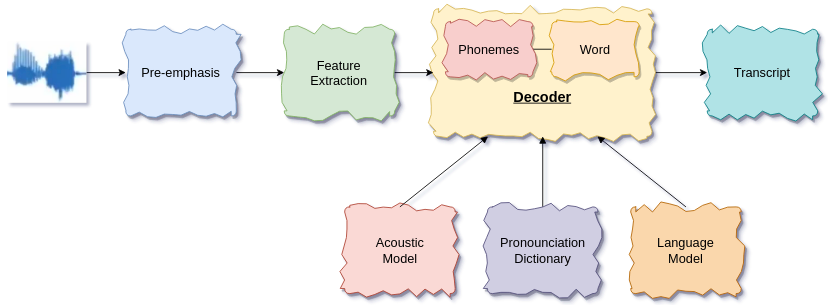
\includegraphics[width=0.75\linewidth]{ASR/images/asr_blocks}
%     \caption{Traditional ASR system blocks diagram}\label{fig:asr_blocks}
% \end{figure}

% \begin{figure}[H]
%     \centering
%     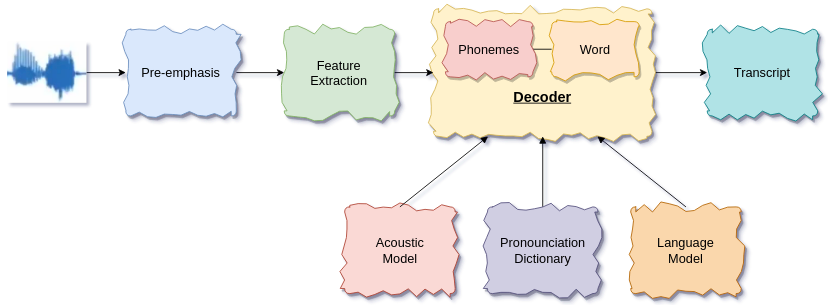
\includegraphics[width=0.75\linewidth]{ASR/images/asr_blocks}
%     \caption{End-to-end ASR system blocks diagram}\label{fig:asr_blocks}
% \end{figure}

\section{The ASR Engine}
The proposed general architecture for the suggested 
ASR engines listed in Table\;\ref{tbl:asr_engines} 
is constructed with a CNN front-end connected to
a self-attention based transformer, 
implying an Encoder-Decoder infrastructure. 

% Joint CTC (Connectionist Temporal Classification) + Seq2Seq (Sequence-To-Sequence) Transformer (self-attention) based.

\subsection{Front-End}
\begin{figure}[H]
    \centering
    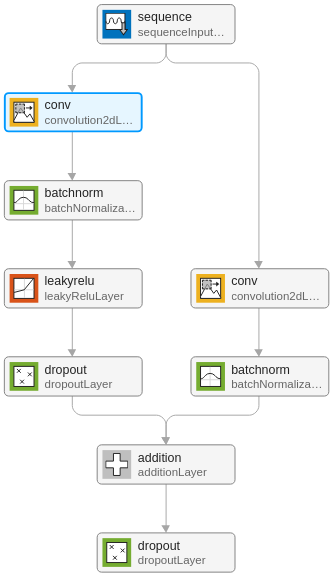
\includegraphics[width=0.45\linewidth]{ASR/images/single_convblock}
    \caption{CNN front-end general ConvBlock architecture.}\label{fig:transformer_cnn_convblock}
    % \source{Adapted from \citep{ADI_MIMO}}
\end{figure}

\subsection{Transformer}
A transformer is a self-attention Encoder-Decoder
based model whose architecture is
shown in Figure\;\ref{fig:transformer_blocks}.
The left side is the Encoder, and the right
side is the Decoder.

\begin{figure}[H]
    \centering
    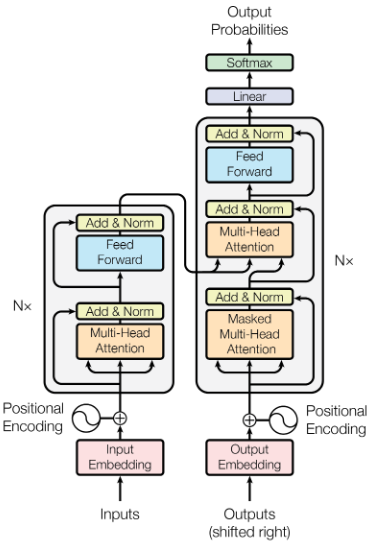
\includegraphics[width=0.75\linewidth]{ASR/images/transformer_blocks}
    \caption{Transformer}\label{fig:transformer_blocks}
    \source{Adapted from ``Attention Is All You Need'' \cite{vaswani2017attention}}
\end{figure}

The attention function that translates 
the Query \((Q)\) and the keys-values pairs \((K)\), \((V)\),
respectively, can be implemented in Scaled Dot-Product Attention
or in Multi-Head Attention.
The transformer backend used in this work is
a Multi-Head Attention-based utilizing
eight heads in the attention model. The Encoder 
and decoder parts consist of a variable
number of linear layers ranging from four to eight.
The activation function used
with the transformer is the \emph{GELU} (Gaussian
Error Linear Unit).

\subsection{CTC}
The CTC loss is the negative logarithm of the probabilities that resulted
from the CTC algorithm. Minimizing the CTC loss is in fact selecting
the characters that end up with the highest probabilities. 
As a result, the predicted label collapses, 
meaning that any repeated characters not separated by the 
``blank'' character unite into a single character.

\begin{equation}
    \hat{\theta} = arg \min_{\theta} - \sum_{i=1}^{N} \left[ \sum p\left( \pi | x^{(i)}; \theta \right) \right]
\end{equation}

\subsection{Seq2Seq}
\begin{equation}
    \ell(x, y) = L = \left\{ \ell_{_{1}}, \ell_{_{2}}, ..., \ell_{_{N}} \right\} 
\end{equation}
\begin{equation}
    \ell_{_{n}} = y_{_{n}} \left[ \log \left( y_{_{n}} \right) - x_{_{n}} \right]
\end{equation}
The kldiv loss also can be reduced over the mini-batch size, as follows:
\begin{equation}
    \ell(x, y) = \begin{cases}
        \frac{\sum {L}}{batch\_size}, & red=meanbatch \\
        \sum {L}, & red=sum
    \end{cases}
\end{equation}
Combining both the CTC and the Seq2Seq components,
the engine's loss function used for training is as follows:
\begin{equation}
    \ell = \omega_{_{ctc}}  \ell_{_{ctc}} + (1 - \omega_{_{ctc}}) \cdot \ell_{_{seq}}
\end{equation}
Where \(\omega_{_{ctc}}\) is set to 0.3 and a greater weight of 0.7 is
given to the Seq2Seq loss \(\ell_{_{seq}}\).

% Feature Extraction:
% N FFT = 400
% N Filters (Mels) = 80

% \subsection{Training Process}
% Batch: 5
% num samples = 150000


% \subsection{FB Feature}
% CNN :
% input shape: (8, 10, 80)
% num blocks: 3
% num layers per block: 1
% out channels: (128, 200, 256)
% kernel sizes: (3, 3, 1)
% strides: (2, 2, 1)
% residuals: (False, False, False)

% Transformer input size = 80 / 2(Cnn1) / 2(Cnn2) · 256
%                             = 20 · 256 = 5120
                            
% \subsection{MFCC + deltas Features}
% Transformer input size = 60 / 2(Cnn1) / 2(Cnn2) · 256
%                             = 15 · 256 = 3840

% \subsection{Validation Process}

% \subsection{Testing Process}

% Transformer Encoder
% Transformer Decoder + (CTC/ATT joint) beamsearch

% Tokens: unigram 500



% \subsection{RNN Based Transducer}

% \subsection{AED CTC Seq2Seq}

\begin{table}[H]
    % for more info see: https://www.overleaf.com/learn/latex/tables
    % \centering
    \hspace*{-2.8cm}
    \arrayrulecolor{ytblborder}
\begin{tabular}{ !{\color{ytblborder}\vrule}l!{\color{ytblborder}\vrule}lrllrr| } 
    \hline

    \hline
    \rowcolor{ytblcaption} \color{white}\bf{Id(seed)} 
    & \color{white}\bf{Feature(s)} 
    & \color{white}\bf{Params} 
    & \color{white}\bf{Scale} 
    & \color{white}\bf{Fbank} 
    & \color{white}\bf{\#Filt.} 
    & \color{white}\bf{\#Coeff.} \\
    % & \color{white}\bf{ORM} 
    % & \color{white}\bf{Clean} \\
    \hline

    \hline\hline
    \rowcolor{wtbl}\multicolumn{7}{|c|}{\bf{Root Mean Cepstral Coefficients}}   \\
    \hline

    \hline
    \rowcolor{ytbl}  \#1(5)  
        & RMFCC(0.1), \(\Delta\), \(\Delta\Delta\) 
        & 146.2M
        & Mel 
        & Bartlett
        & 80 
        & 20 \\
    \hline
    
    \hline
    \rowcolor{wtbl}  \#2(15)  
        & RMFCC(0.08), \(\Delta\), \(\Delta\Delta\) 
        & 146.2M
        & Mel 
        & Bartlett
        & 80 
        & 20 \\
    \hline
    
    \hline
    \rowcolor{ytbl}  \#3(12)  
        & RBFCC(0.1), \(\Delta\), \(\Delta\Delta\) 
        & 146.0M
        & Bark 
        & Bartlett
        & 28 
        & 18 \\
    \hline

    \hline
    \rowcolor{wtbl}  \#4(13)  
        & RGFCC(0.1), \(\Delta\), \(\Delta\Delta\) 
        & 146.0M
        & ERB
        & Gammatone
        & 28 
        & 18 \\
    \hline

    \hline\hline
    \rowcolor{wtbl}\multicolumn{7}{|c|}{\bf{Conventional Cepstral Coefficients}}   \\
    \hline

    \hline
    \rowcolor{ytbl}  \#5(70)  
        & MFCC, \(\Delta\), \(\Delta\Delta\) 
        & 146.2M
        & Mel 
        & Bartlett
        & 80 
        & 20 \\
    \hline
    
    \hline
    \rowcolor{wtbl}  \#6(72)  
        & MFCC, \(\Delta\), \(\Delta\Delta\) 
        & 146.0M
        & Mel 
        & Bartlett
        & 28 
        & 18 \\
    \hline

    \hline
    \rowcolor{ytbl}  \#7(22)  
        & MFCC, \(\Delta\), \(\Delta\Delta\) 
        & 146.0M
        & Bark 
        & Bartlett
        & 28 
        & 18 \\
    \hline

    \hline
    \rowcolor{wtbl}  \#8(23)  
        & MFCC, \(\Delta\), \(\Delta\Delta\) 
        & 146.0M
        & ERB
        & Gammatone
        & 28 
        & 18 \\
    \hline

    \hline
    \rowcolor{ytbl}  \#9(100)  
        & MFCC, \(\Delta\), \(\Delta\Delta\), Context(3, 3)
        & 78.8M
        & Mel 
        & Bartlett
        & 26 
        & 26 \\
    \hline

    \hline
    \rowcolor{wtbl}  \#10(101)
        & MFCC, \(\Delta\), \(\Delta\Delta\), Context(3, 3)
        & 78.8M
        & Mel Approx.
        & Bartlett
        & 26 
        & 26 \\
    \hline

    \hline
\end{tabular}
\arrayrulecolor{black}
\caption{ASR Engines Table}
\label{tbl:asr_engines}
\end{table}
\vspace{-0.7cm}
ASR engines 100, 101 were heavily 
optimized in terms of the neural network structures, 
leading to smaller models having two times fewer learnable parameters.
For comparison, differences between ASR engines 101
and 72 are summarized in
Table\;\ref{tbl:engine_101_72}.
\begin{table}[H]
    % for more info see: https://www.overleaf.com/learn/latex/tables
    \centering
    % \hspace*{-2.8cm}
    \arrayrulecolor{ytblborder}
\begin{tabular}{ !{\color{ytblborder}\vrule}l!{\color{ytblborder}\vrule}cc| } 
    \hline

    \hline
    \rowcolor{ytblcaption} \color{white}\bf{Parameter} 
    & \color{white}\bf{Engine \#101} 
    & \color{white}\bf{Engine \#72} \\
    % & \color{white}\bf{ORM} 
    % & \color{white}\bf{Clean} \\
    \hline

    \hline\hline
    \rowcolor{wtbl}\multicolumn{3}{|c|}{\bf{CNN Settings}}   \\
    \hline

    \hline
    \rowcolor{ytbl}  CNN Blocks [\#]  
        & 3 
        & 3 \\
    \hline
    
    \hline
    \rowcolor{wtbl}  CNN Shapes  
        & [64, 100, 128]
        & [128, 200, 256] \\
    \hline

    \hline\hline
    \rowcolor{wtbl}\multicolumn{3}{|c|}{\bf{Transformer Settings}}   \\
    \hline

    \hline
    \rowcolor{ytbl}  FFN layers  
        & 2048
        & 3072 \\
    \hline

    \hline
    \rowcolor{wtbl}  Input size
        & 2560
        & 3584 \\
    \hline

    \hline
    \rowcolor{ytbl}  Enc. layers
        & 8
        & 12 \\
    \hline

    \hline
    \rowcolor{wtbl}  Dec. layers
        & 4
        & 6 \\
    \hline


    \hline\hline
    \rowcolor{wtbl}\multicolumn{3}{|c|}{\bf{Implementation Settings}}   \\
    \hline

    \hline
    \rowcolor{ytbl}  Filters [\#] 
        & 26
        & 28 \\
    \hline

    \hline
    \rowcolor{wtbl} Coeff. [\#]  
        & 2048
        & 3072 \\
    \hline

    \hline
    \rowcolor{ytbl} Precision  
        & U16/8
        & FP64 \\
    \hline

    \hline
\end{tabular}
\arrayrulecolor{black}
\caption{ASR engines \#101, \#72 comparison table}
\label{tbl:engine_101_72}
\end{table}


% \begin{figure}[H]
%     \centering
%     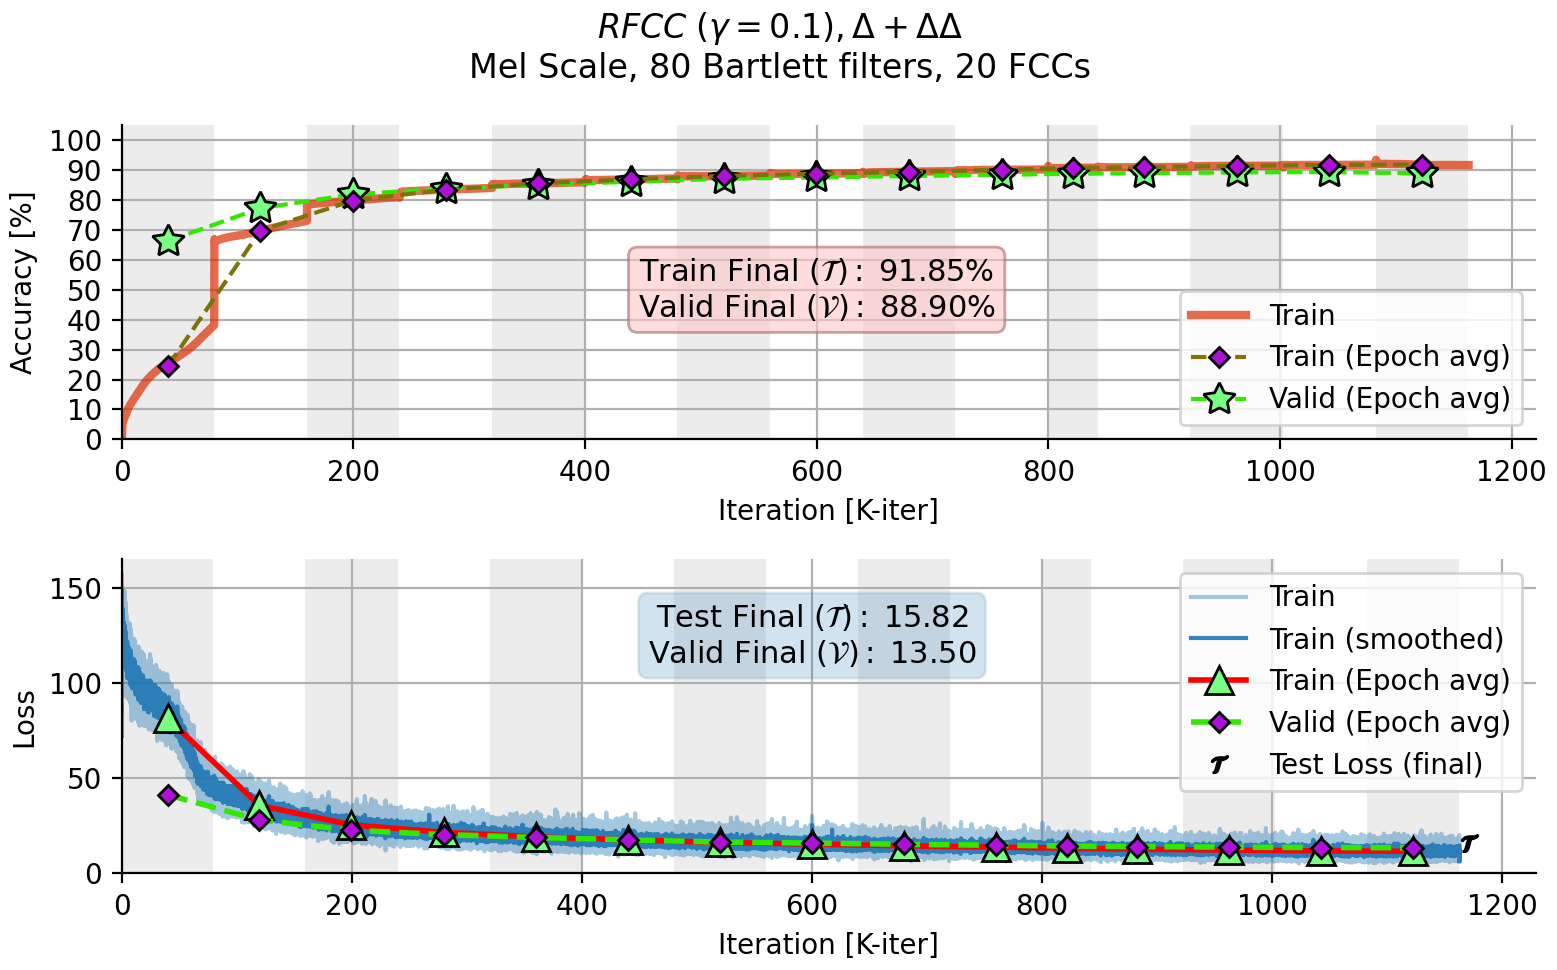
\includegraphics[width=0.75\linewidth]{Experiments/images/asr_5}
%     \caption{ASR \#5 training }\label{fig:asr_5}
% \end{figure}

% \begin{figure}[H]
%     \centering
%     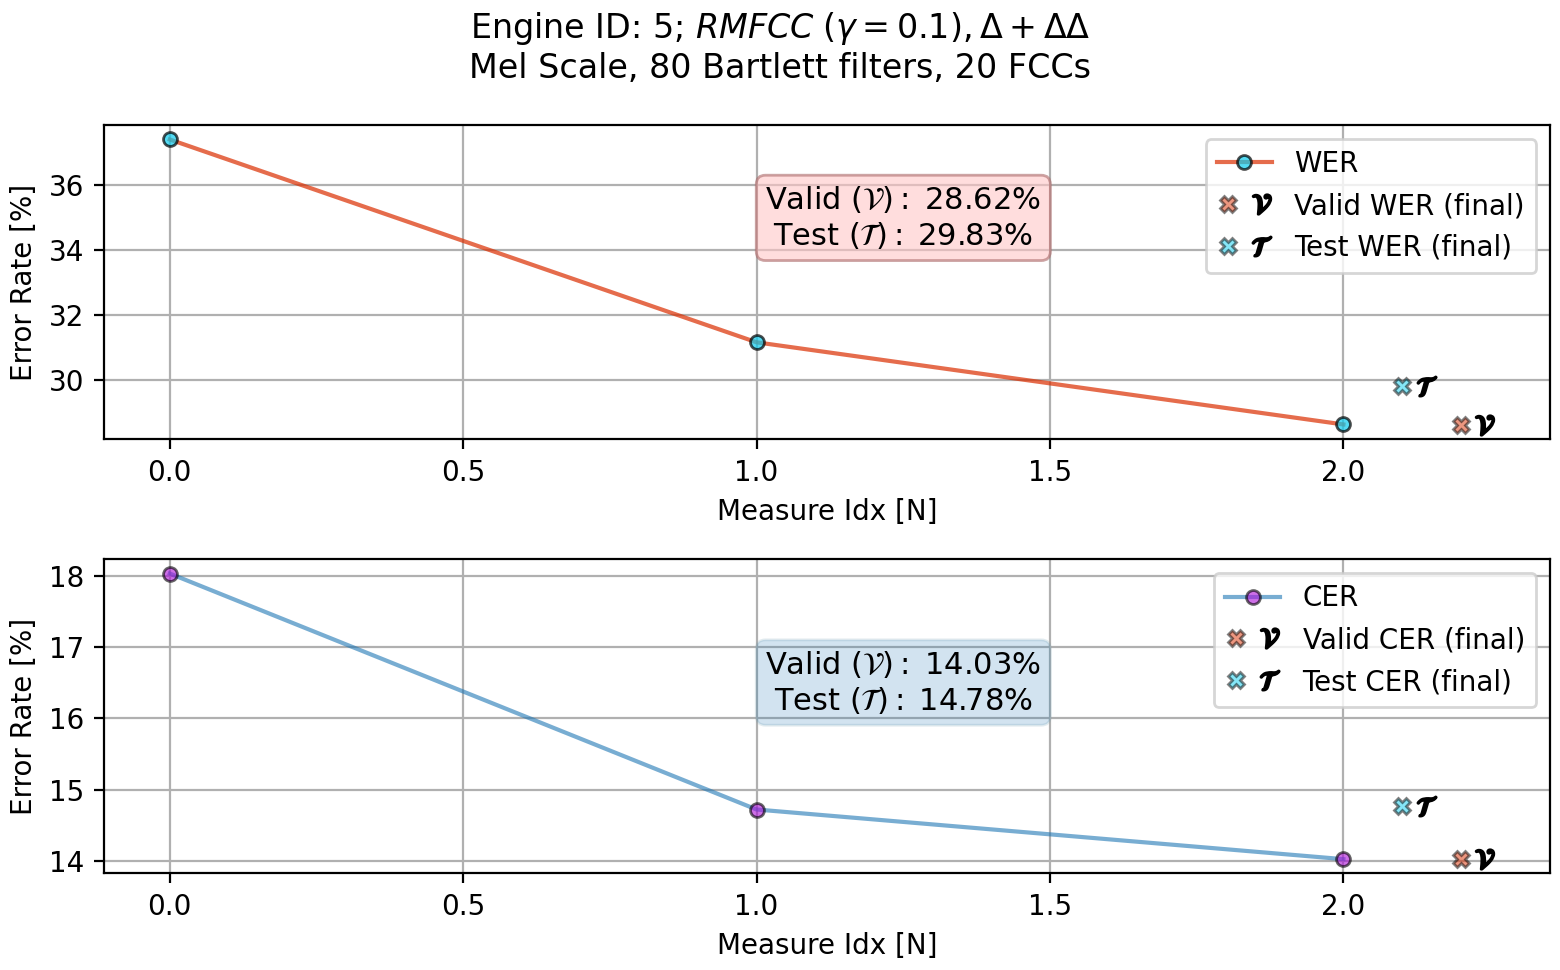
\includegraphics[width=0.75\linewidth]{ASR/images/asr5_wer.png}
%     \caption{ASR \#5 WER, CER results}\label{fig:asr5_wer}
% \end{figure}

\subsection{Trained Engines}
\subsubsection{ASR Engine \#5 --- RMFCC(0.1), \(\Delta,\;\Delta\Delta\)}
ASR engine \#5 had been trained over fifteen epochs,
against a \(400K\) recordings table, with a minibatch size 
of four per iteration. 
The engine was trained against the RMFCCs, 
when \(\gamma=0.1\),
with the \(\Delta,\;\Delta\Delta\) features, utilizing
the Log-Mel scale. A preprocessing STFT enframing
block was set with
80 Bartlett filters for each T-F bin.
Overall the number of features
per T-F unit is 20 cepstral coefficients plus the
first and second derivatives.
Figure\;\ref{fig:asr_5} shows ASR engine \#5 training results
for the test and validation subsets.
In Figure\;\ref{fig:asr5_wer},
we present the evaluated WER and CER measures
taken every five epochs during the training process.

\begin{figure}[H]
    \centering
    \subfloat[\label{fig:asr_5}]{%
       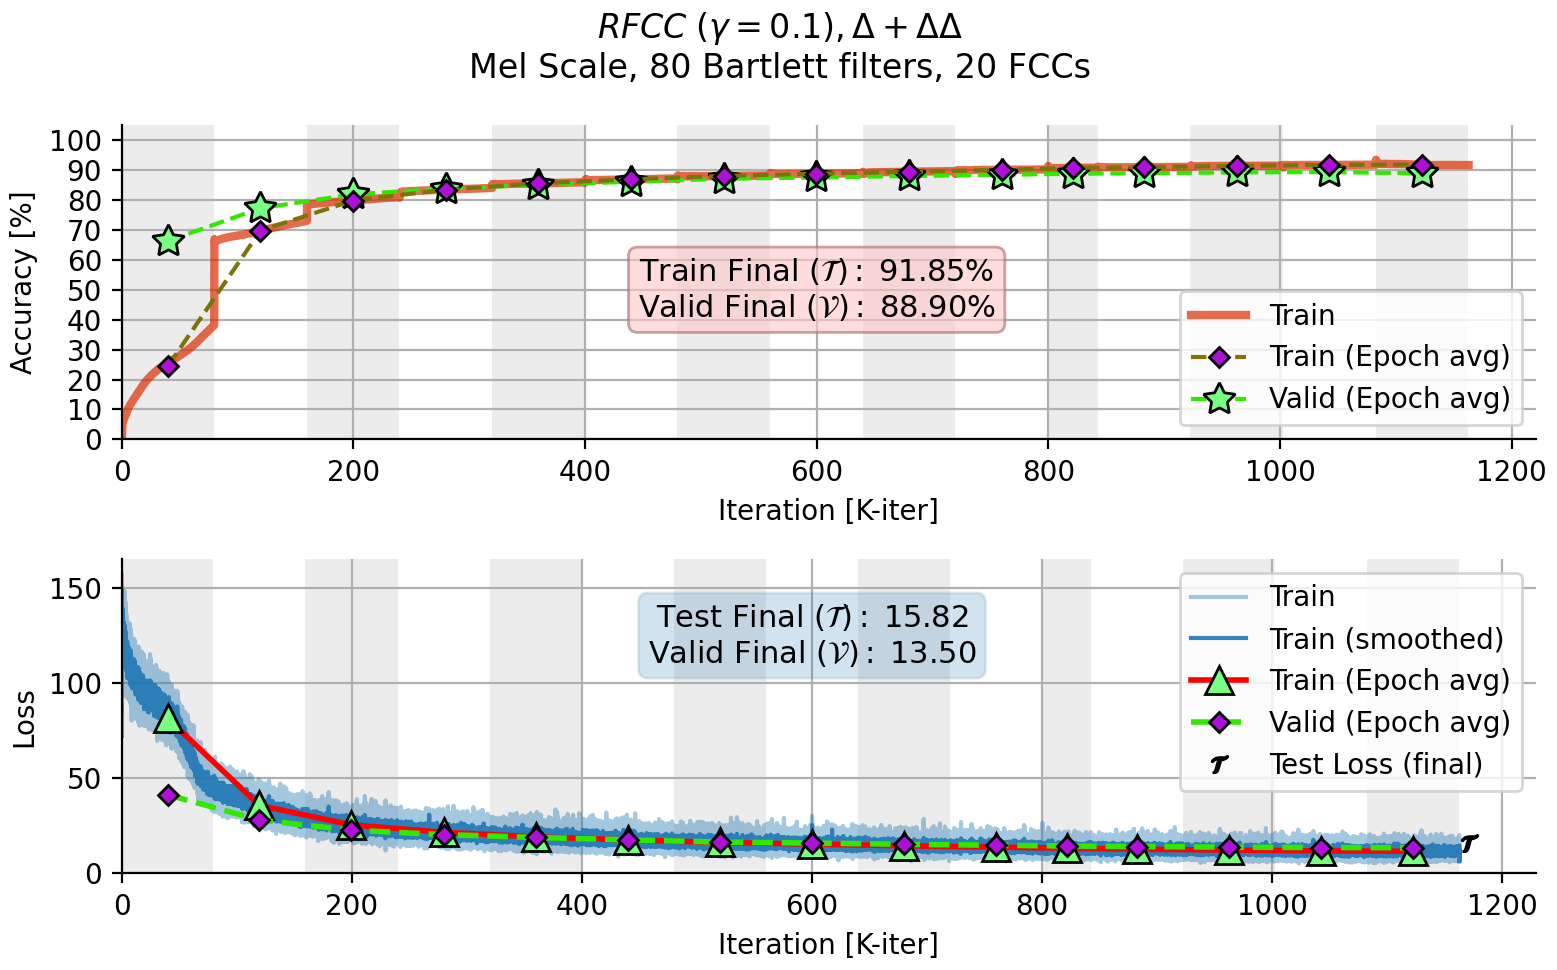
\includegraphics[width=0.85\linewidth]{Experiments/images/asr_5}}
    \\
    \vspace{-0.3cm}
    \subfloat[\label{fig:asr5_wer}]{%
        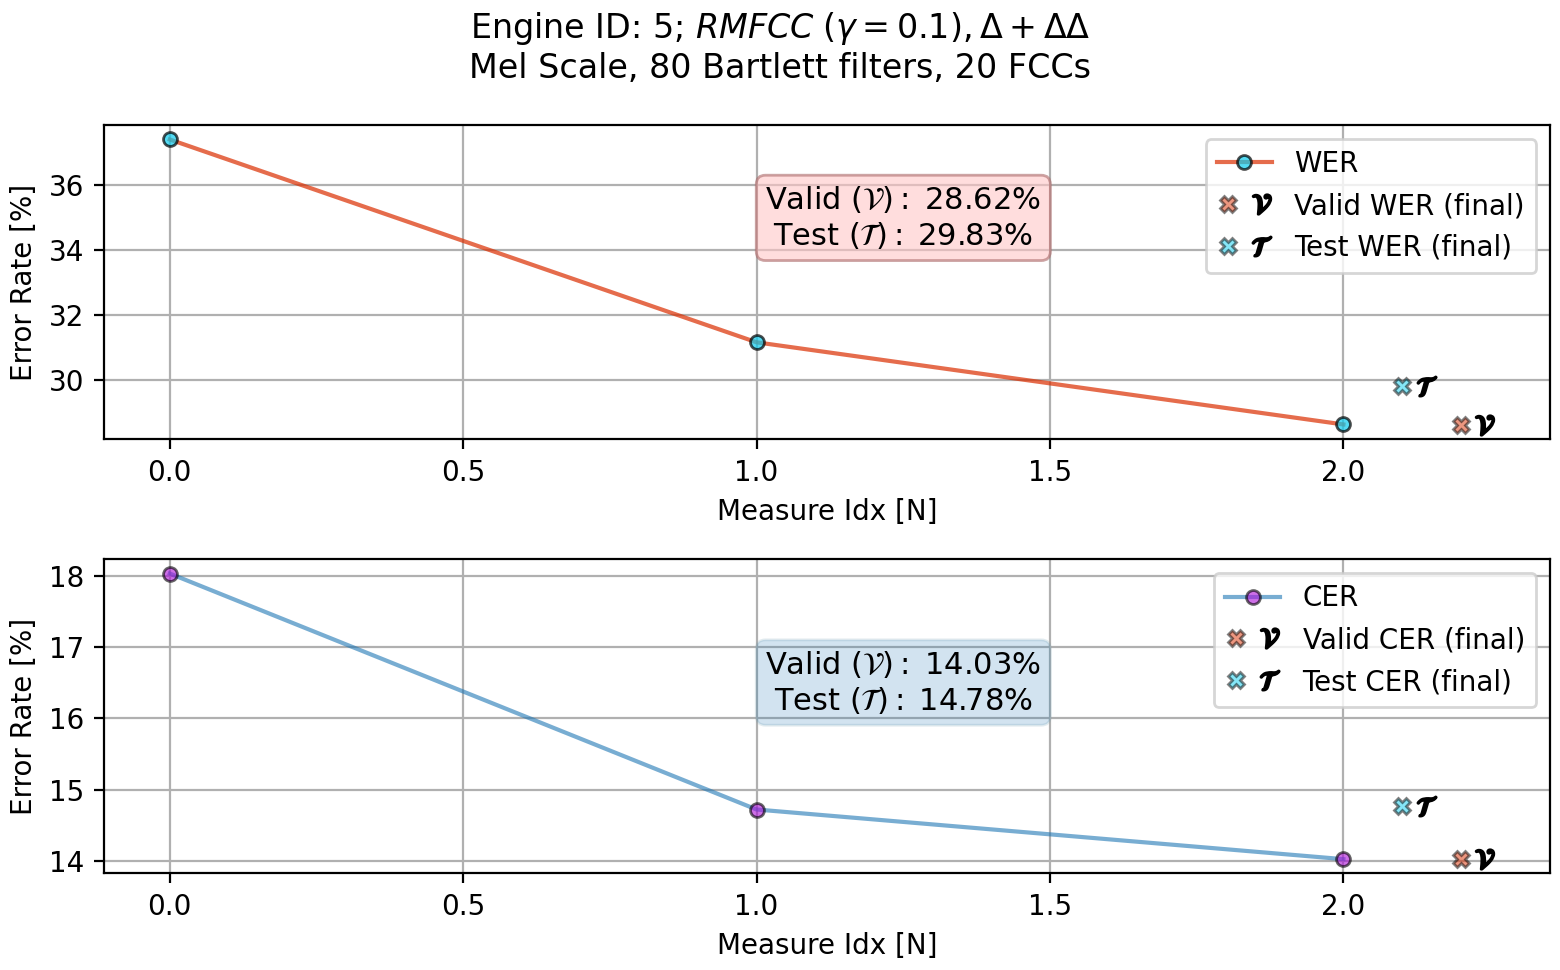
\includegraphics[width=0.85\linewidth]{ASR/images/asr5_wer}}
    \caption{(a) ASR \#5 training accuracy and loss plot;\;\;
        (b) ASR \#5 WER, CER evaluation plot.}\label{fig:asr5_wer_subplot} 
\end{figure}

\begin{figure}[H]
    \centering
    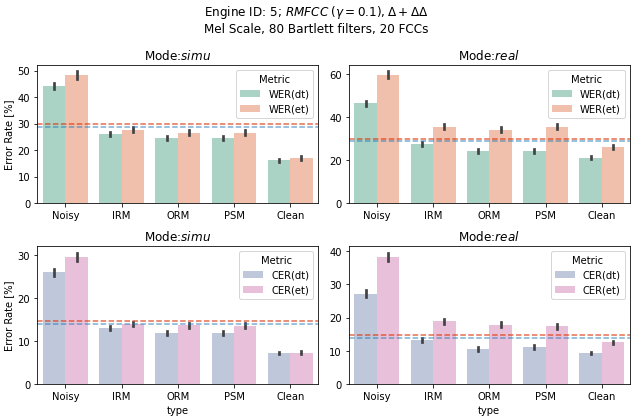
\includegraphics[width=0.95\linewidth]{ASR/images/asr5_wer_masks.png}
    \caption{ASR \#5 WER, CER vs. T-F masks, noisy and clean inputs}\label{fig:asr5_wer_masks}
\end{figure}

In Figure\;\ref{fig:asr5_wer_masks}, we present the engine's
results in terms of WER and CER per each subset of
the multi microphone CHiME dataset.
This figure emphasizes the comparison between the
four T-F masking algorithms. Results are plotted side by side with
the evaluated noisy mixture and clean speech metrics as reference.
Two horizontal lines, red and blue, are stretched across the x-axis
of each plot. These lines mark the plot's metric, 
whether WER or CER, taken from the training evaluations of 
CommonVoice datasets validation and test subsets.
The red line is for the test measurement
and the blue line marks the validation measurement.

\subsubsection{ASR Engine \#15 --- RMFCC(0.08), \(\Delta,\;\Delta\Delta\)}
ASR engine \#15 had been trained over fifteen epochs,
along a \(400K\) recordings table, with a minibatch size 
of four per iteration. 
The engine was trained against the RMFCCs,
utilizing the Log-Mel scale with the \(\Delta,\;\Delta\Delta\) features.
Gamma has been set to
\(\gamma=0.08\), as this setting proved to be
the optimized value as stated in \cite{rmfcc1}.
The rest of the settings are similar to
ASR engine \#5. 
\bigskip

Figures\;\ref{fig:asr_15} and \;\ref{fig:asr15_wer} show
the training results of ASR engine \#15 and its
WER and CER benchmarks for the validation and test subsets.
\begin{figure}[H]
    \centering
    \subfloat[\label{fig:asr_15}]{%
       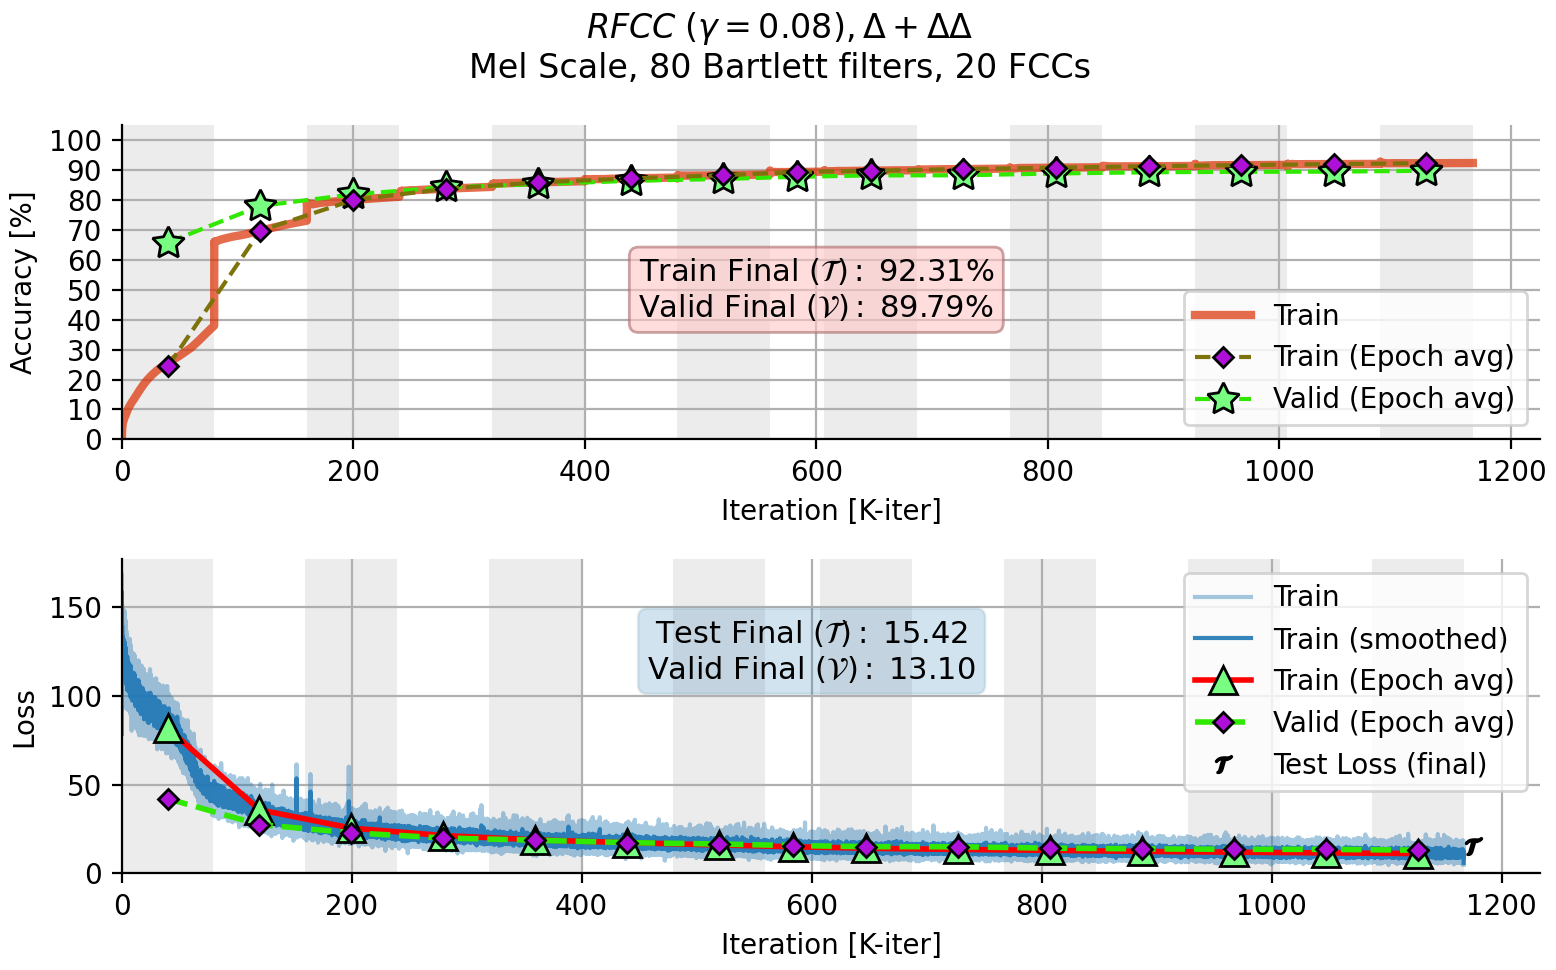
\includegraphics[width=0.85\linewidth]{Experiments/images/asr_15}}
    \\
    \vspace{-0.3cm}
    \subfloat[\label{fig:asr15_wer}]{%
        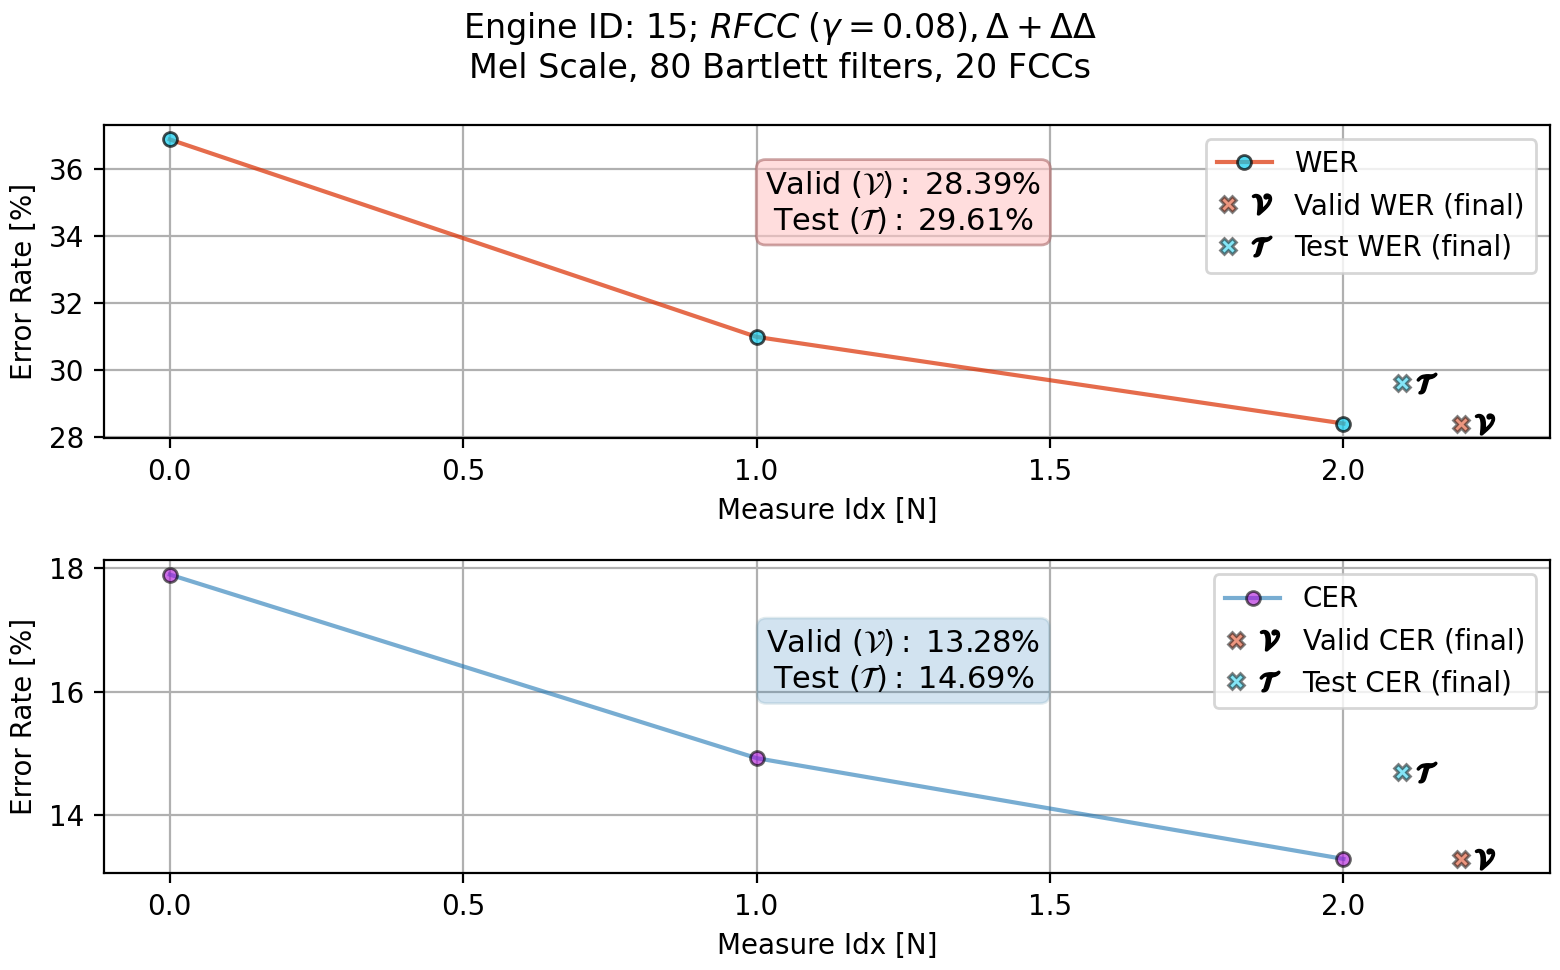
\includegraphics[width=0.85\linewidth]{ASR/images/asr15_wer}}
    \caption{(a) ASR \#15 training accuracy and loss plot;\;\;
        (b) ASR \#15 WER, CER evaluation plot.}\label{fig:asr15_wer_subplot} 
\end{figure}

In Figure\;\ref{fig:asr15_wer_masks} presented the T-F mask based
beamformed enhanced recordings evaluations.
\begin{figure}[H]
    \centering
    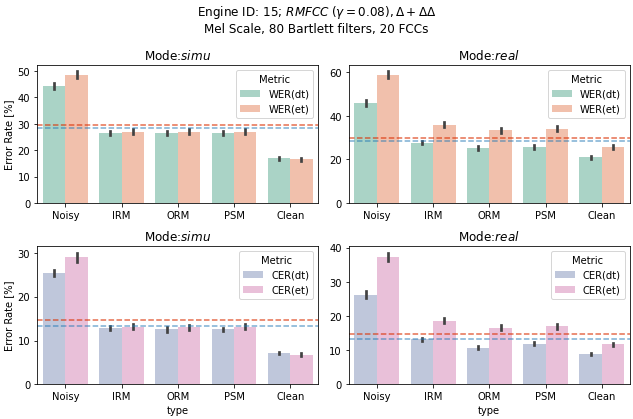
\includegraphics[width=0.95\linewidth]{ASR/images/asr15_wer_masks.png}
    \caption{ASR \#15 WER, CER vs. T-F masks, noisy and clean inputs }\label{fig:asr15_wer_masks}
\end{figure}

\subsubsection{ASR Engine \#12 --- RBFCC(0.1), \(\Delta,\;\Delta\Delta\)}
ASR engine \#12 trained similarly to the previous
engines, \#5 and \#15 but with some distinctions.
The feature set utilizes the Bark scale instead of the previously
used Log-Mel scale, and the number of extracted cepstral 
coefficients has been reduced to 18. 
The number of Bartlett filters per T-F unit has been set
to 28 instead of 80.

\bigskip

Figures\;\ref{fig:asr_12} and \;\ref{fig:asr12_wer} show
the training results, and Figure\;\ref{fig:asr12_wer_masks}
presents the beamforming effect per T-F algorithm, compared to 
the noisy mixture and the clean speech references.
\begin{figure}[H]
    \centering
    \subfloat[\label{fig:asr_12}]{%
       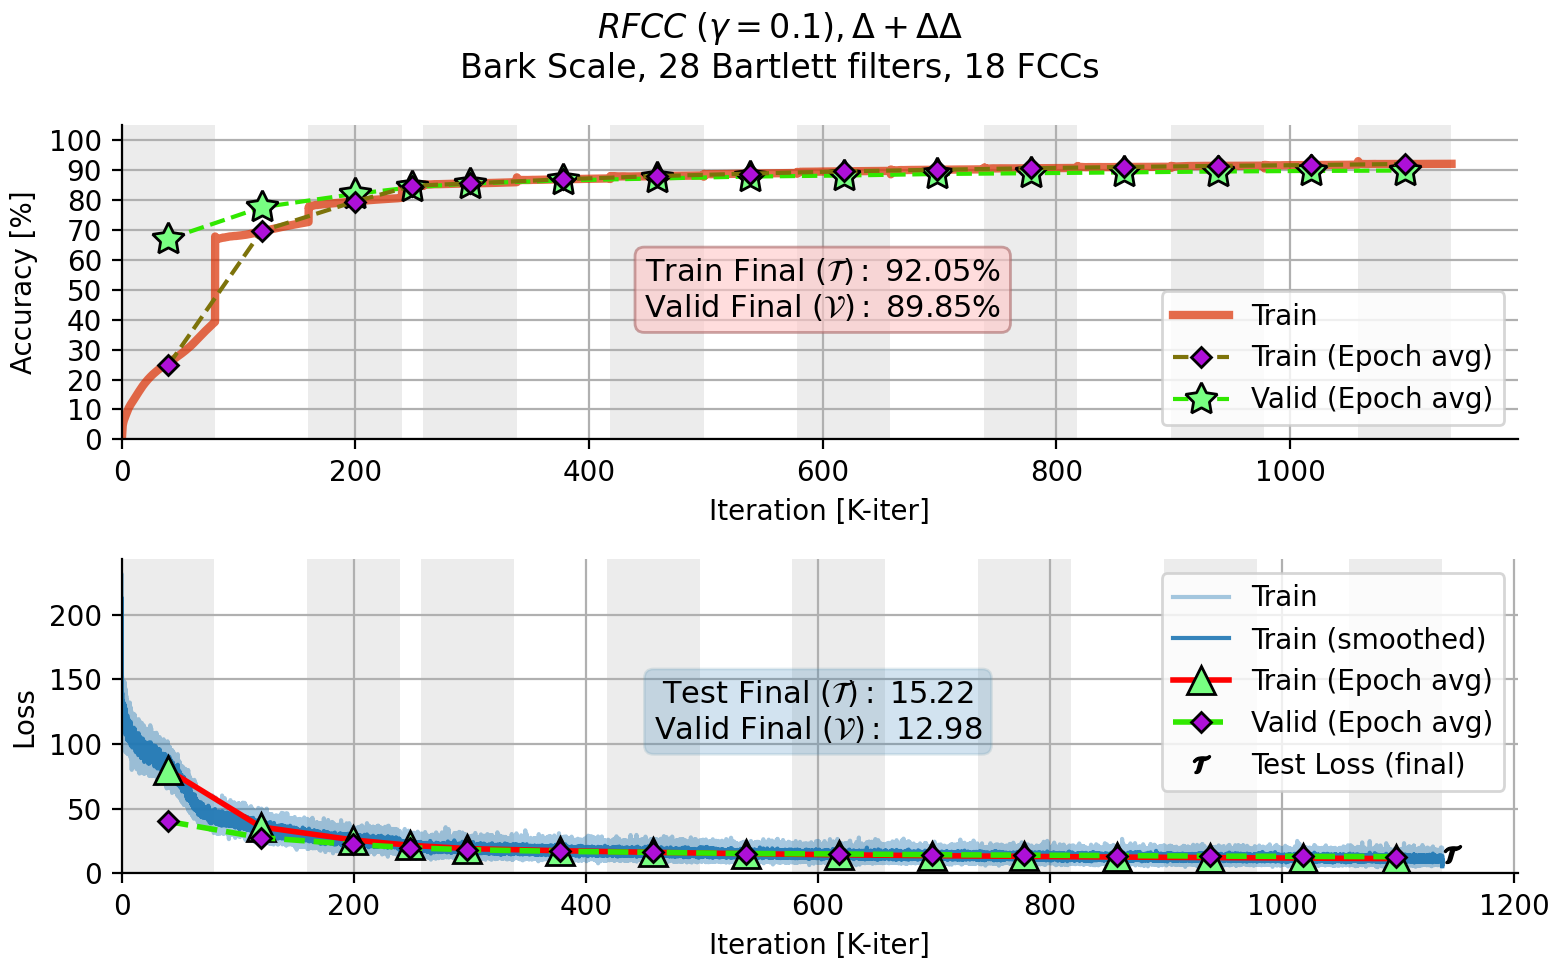
\includegraphics[width=0.85\linewidth]{Experiments/images/asr_12}}
    \\
    \vspace{-0.3cm}
    \subfloat[\label{fig:asr12_wer}]{%
        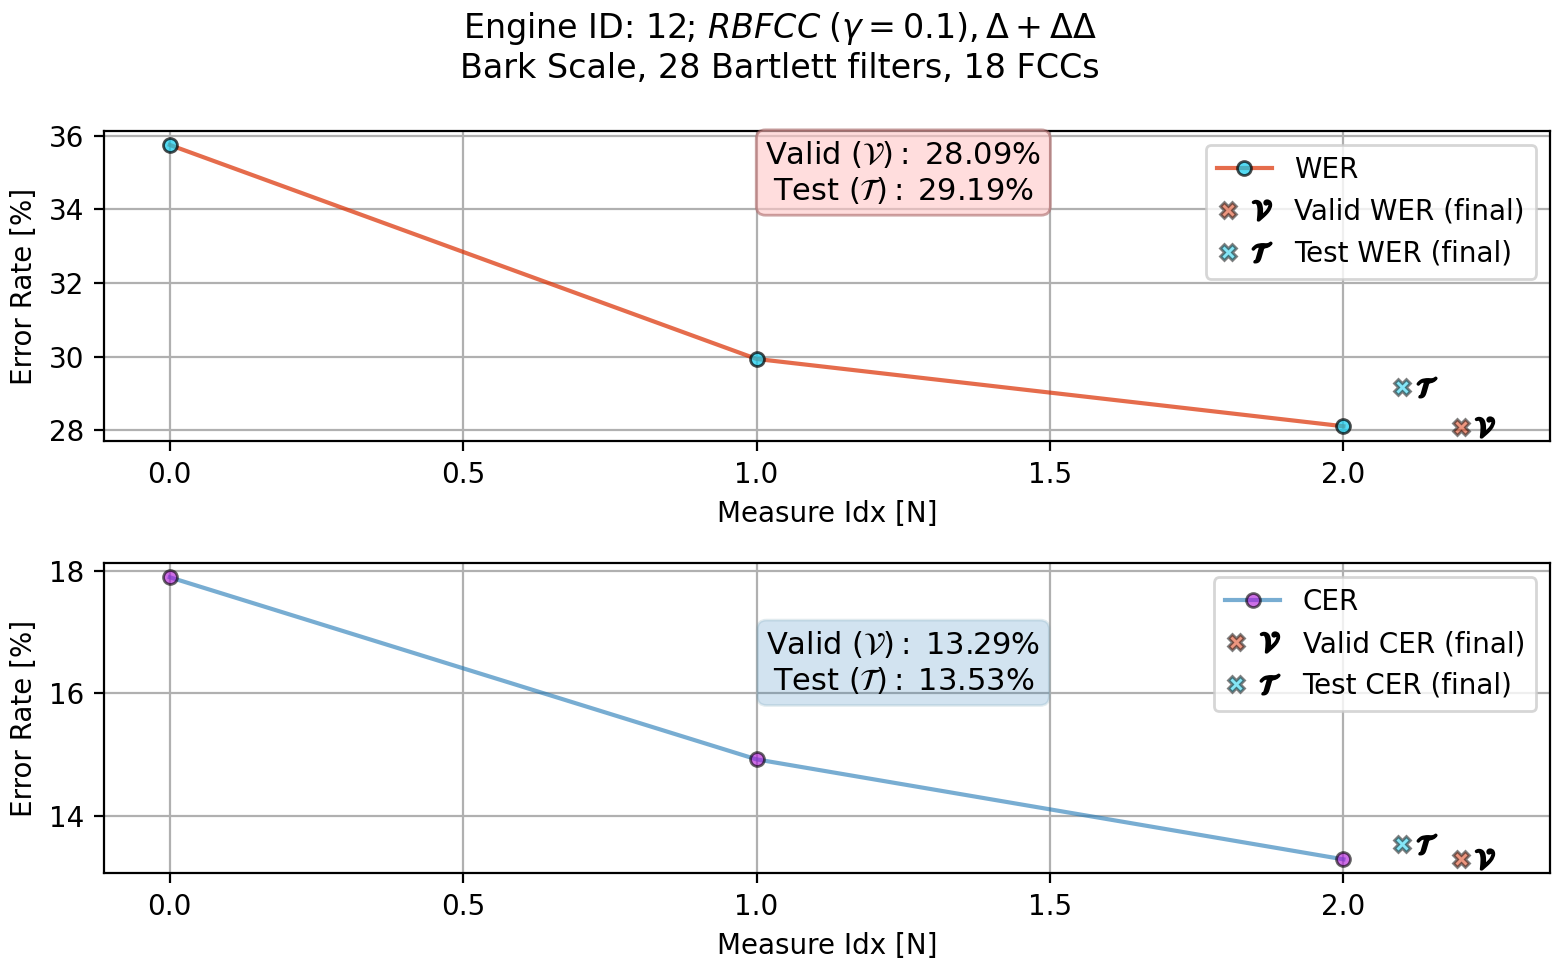
\includegraphics[width=0.85\linewidth]{ASR/images/asr12_wer}}
    \caption{(a) ASR \#12 training accuracy and loss plot;\;\;
        (b) ASR \#12 WER, CER evaluation plot.}\label{fig:asr12_wer_subplot} 
\end{figure}

\begin{figure}[H]
    \centering
    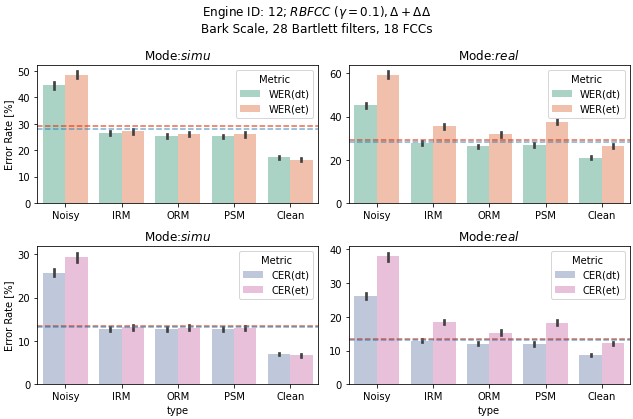
\includegraphics[width=0.95\linewidth]{ASR/images/asr12_wer_masks.png}
    \caption{ASR \#12 WER, CER vs. T-F masks, noisy and clean inputs }\label{fig:asr12_wer_masks}
\end{figure}


% Mel
\subsubsection{ASR Engine \#72 --- MFCC, \(\Delta,\;\Delta\Delta\)}
ASR engine \#72 as opposed to ASR engine \#12, had been trained against
the Mel cepstral coefficients. All the other settings are retained.

\bigskip

Figures\;\ref{fig:asr_72},\;\ref{fig:asr72_wer}, and \ref{fig:asr72_wer_masks}
present the training, evaluation, 
and the T-F based beamforming results, respectively. 
\begin{figure}[H]
    \centering
    \subfloat[\label{fig:asr_72}]{%
       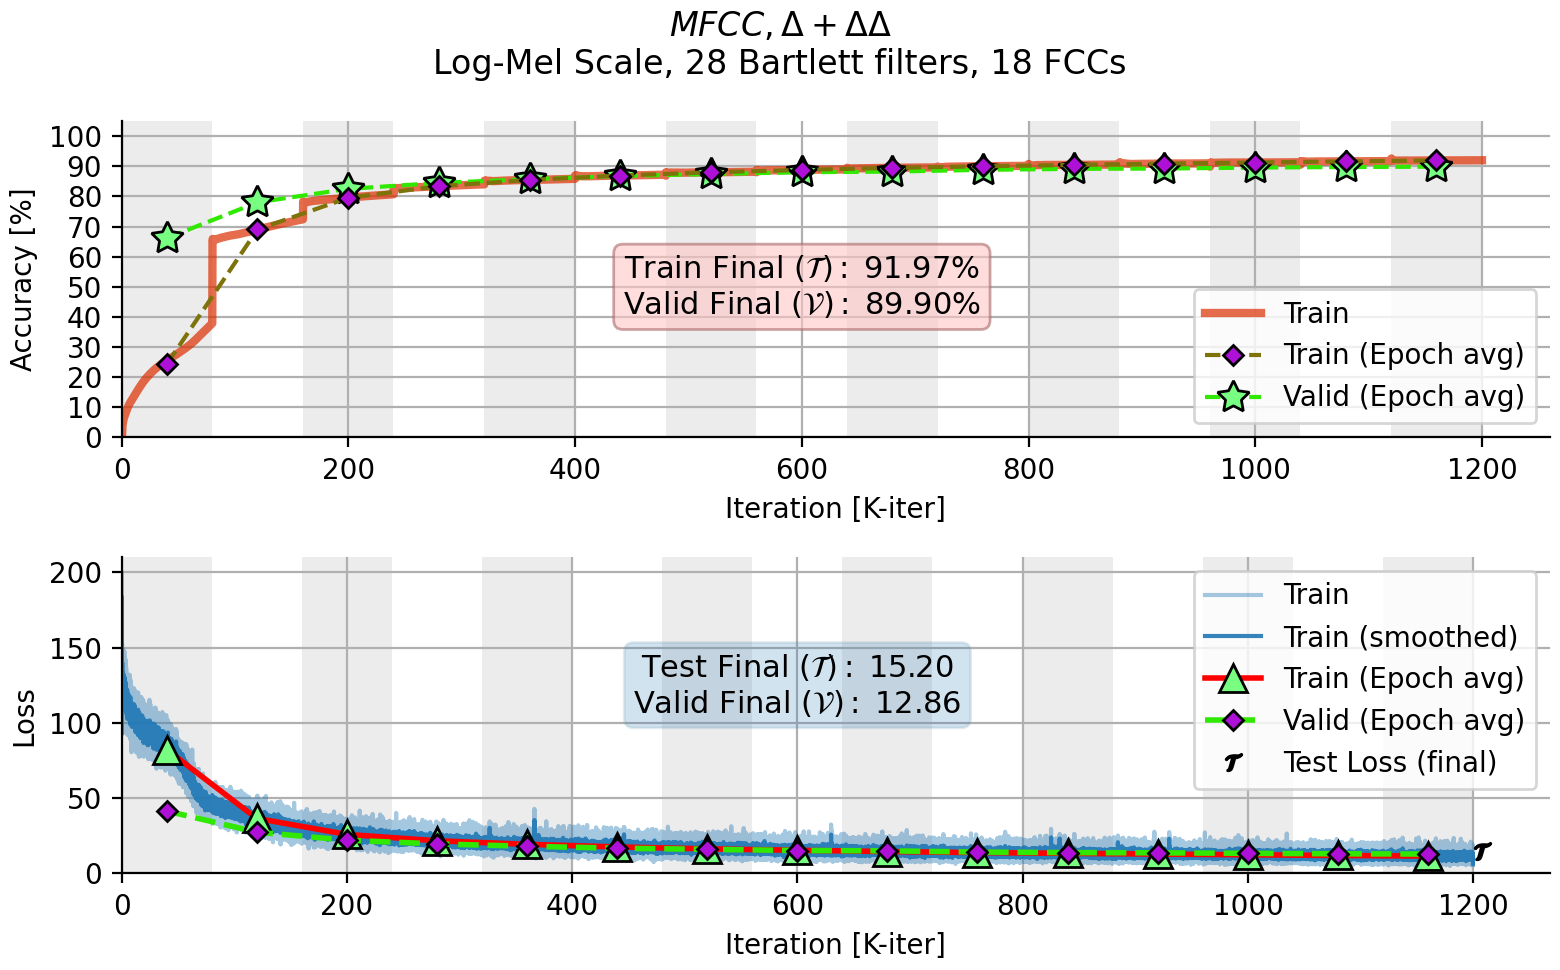
\includegraphics[width=0.85\linewidth]{Experiments/images/asr_72}}
    \\
    \vspace{-0.3cm}
    \subfloat[\label{fig:asr72_wer}]{%
        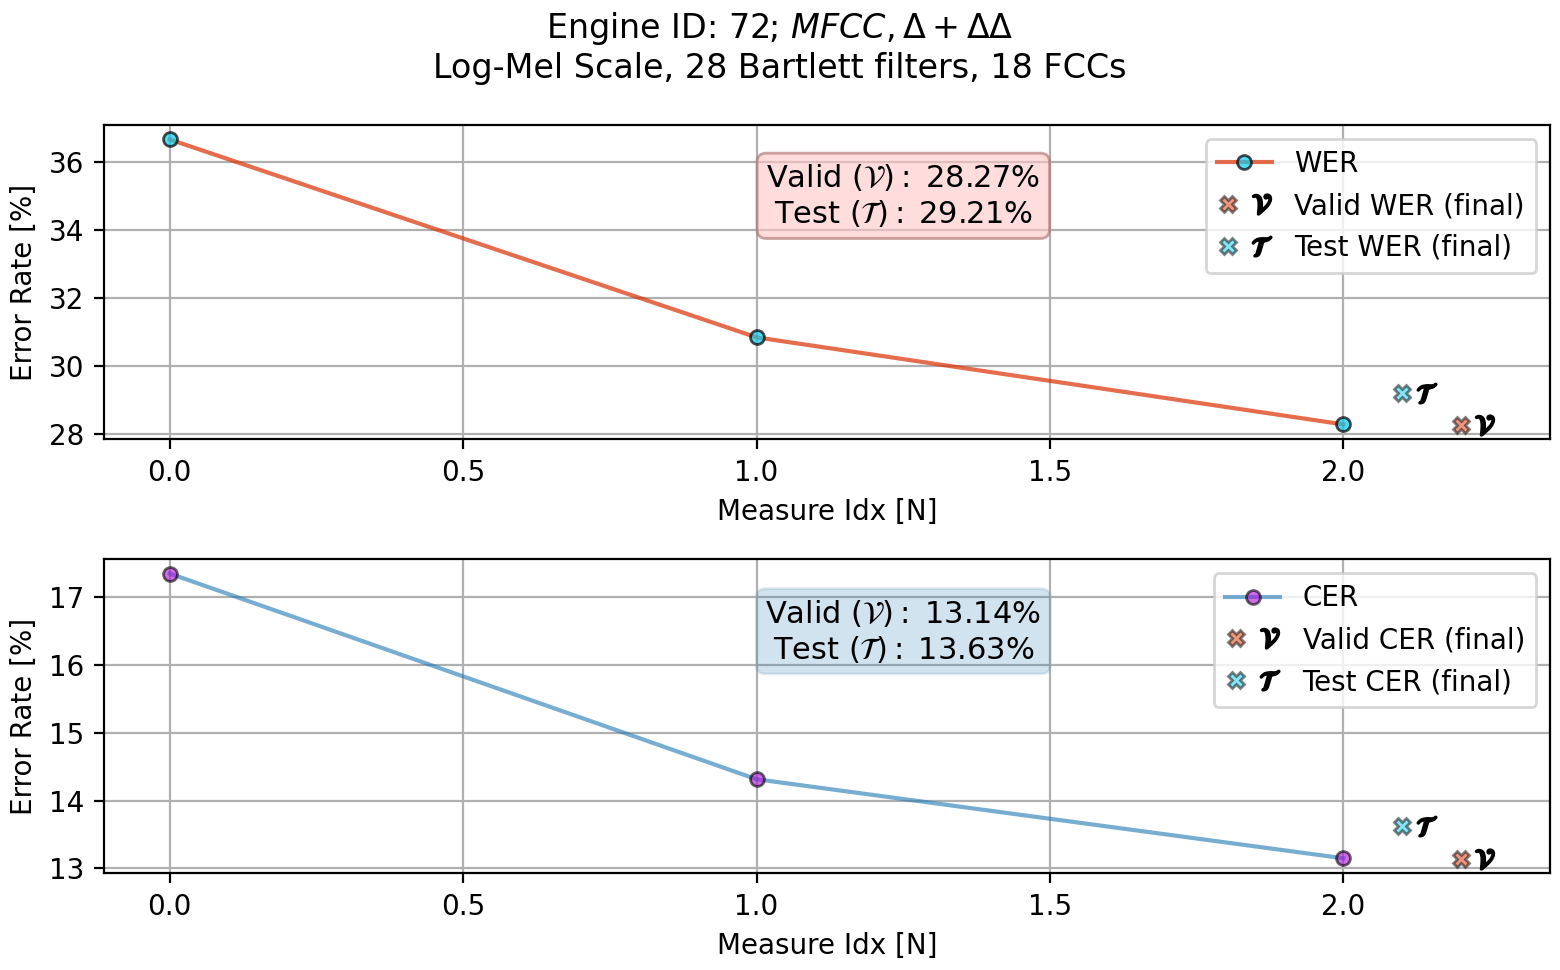
\includegraphics[width=0.85\linewidth]{ASR/images/asr72_wer}}
    \caption{(a) ASR \#72 training accuracy and loss plot;\;\;
        (b) ASR \#72 WER, CER evaluation plot.}\label{fig:asr72_wer_subplot} 
\end{figure}

\begin{figure}[H]
    \centering
    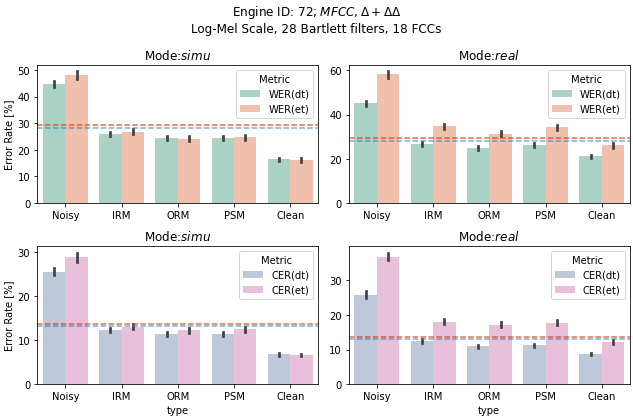
\includegraphics[width=0.95\linewidth]{ASR/images/asr72_wer_masks.png}
    \caption{ASR \#72 WER, CER vs. T-F masks, noisy and clean inputs }\label{fig:asr72_wer_masks}
\end{figure}

\subsubsection{ASR Engine \#100 --- MFCC, \(\Delta,\Delta\Delta\), Context(3, 3)}
ASR engine \#100 is an optimized Log-Mel scale based engine
that has been trained against the Mel cepstral coefficients
with their first and second derivatives. These extracted features
were also taken from six additional adjacent T-F units, three
prior and another three past the currently analyzed unit.
The number of extracted coefficients is set to 26 same as the
total number of Bartlett filters covering the spectrum of each T-F bin.

\bigskip

In contrast to the previous engines, engine \#100
underwent heavy optimization to fit a target hardware device.
In the process, the engine's learnable parameters were quantized
to the U16/8 format from the default 64bit floating point, which is the default.

\bigskip

The training process also changed to train over 40 epochs
with \(100K\) randomly selected recordings from the
entire CommonVoice dataset. The motivation behind
these changes in the training process is to let the model
better generalize in a reasonable training time due to
introducing the additional temporal context 
features vectors and the quantized architecture.

\bigskip

Figures\;\ref{fig:asr_100},\;\ref{fig:asr100_wer}, and \ref{fig:asr100_wer_masks}
present the training, evaluation, and the 
T-F based beamforming results respectively. 

\begin{figure}[H]
    \centering
    \subfloat[\label{fig:asr_100}]{%
       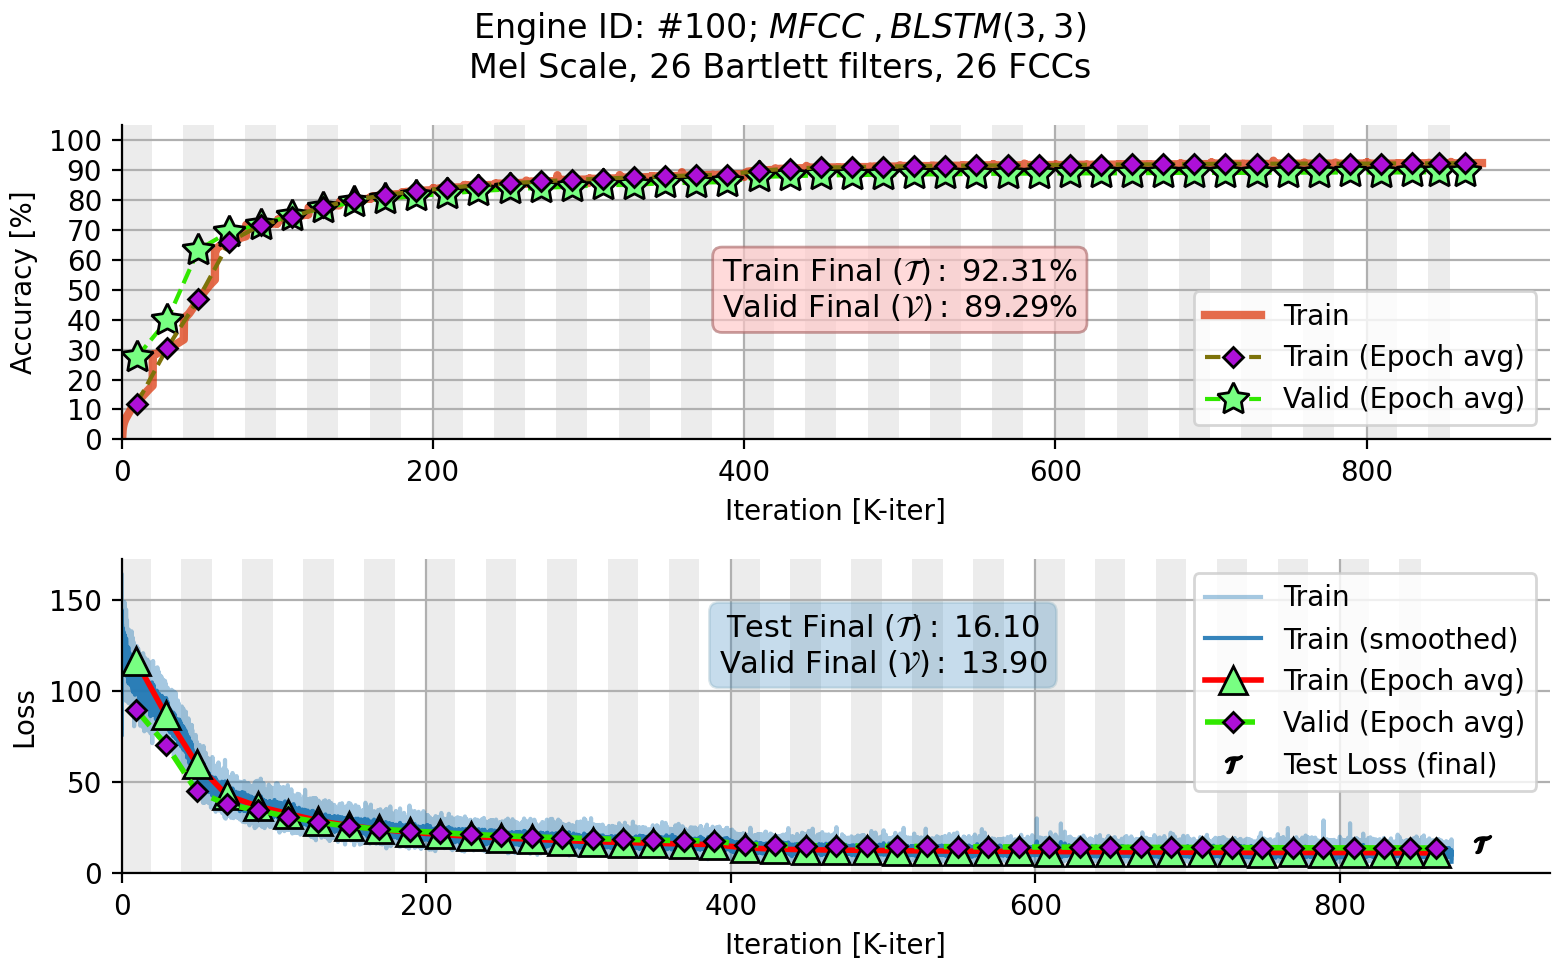
\includegraphics[width=0.85\linewidth]{ASR/images/asr_100}}
    \\
    \vspace{-0.3cm}
    \subfloat[\label{fig:asr100_wer}]{%
        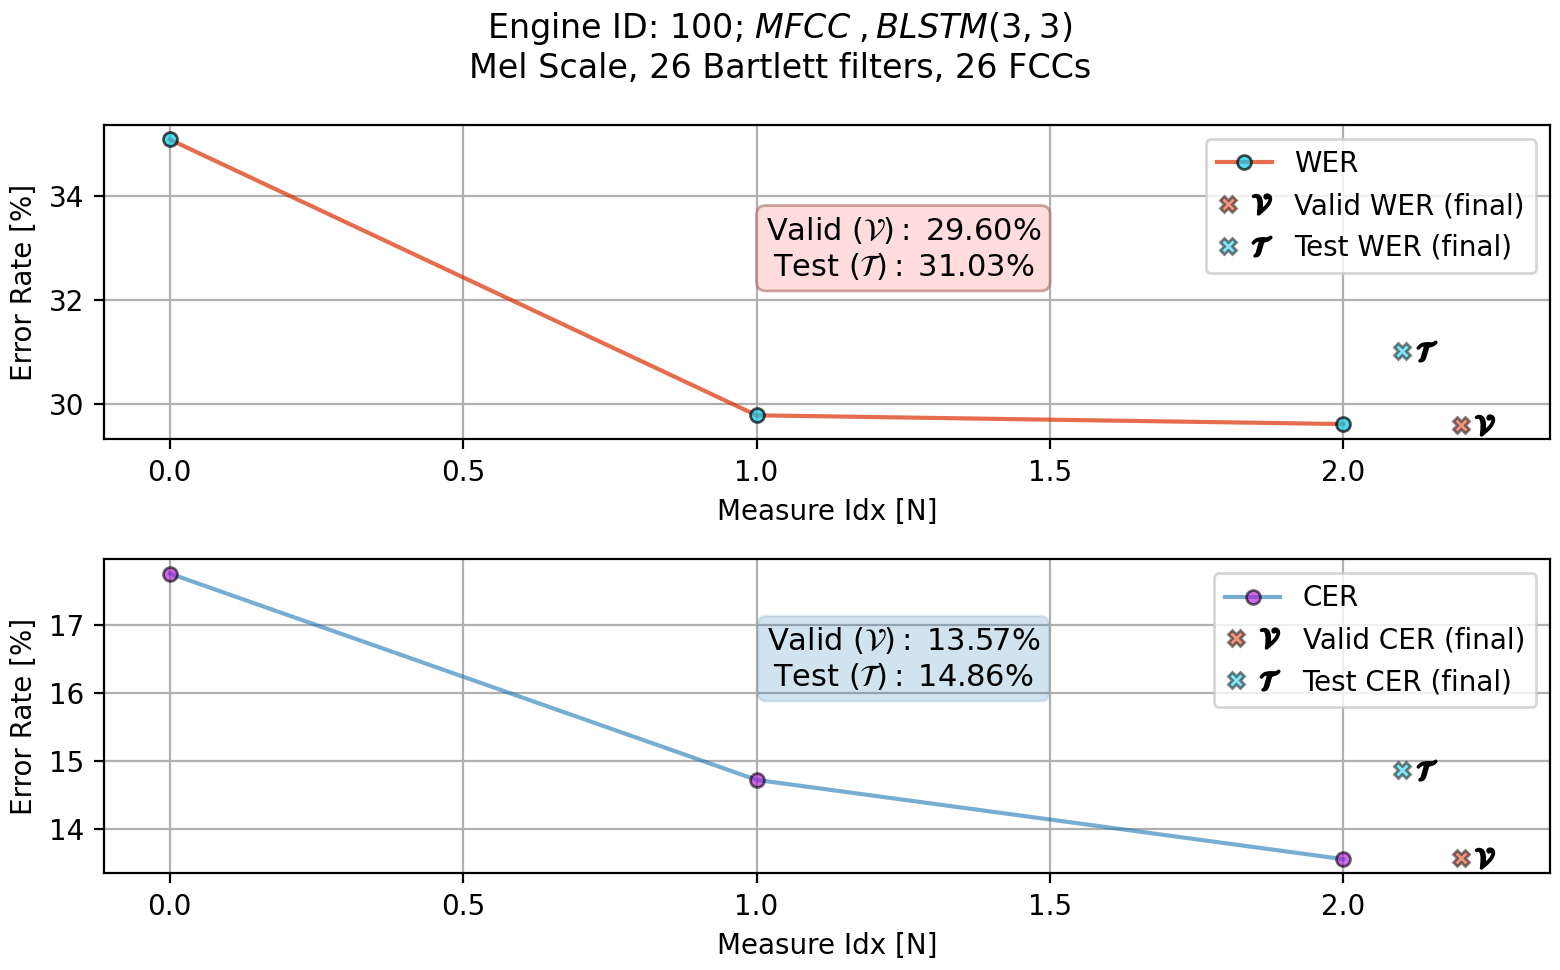
\includegraphics[width=0.85\linewidth]{ASR/images/asr100_wer}}
    \caption{(a) ASR \#100 training accuracy and loss plot;\;\;
        (b) ASR \#100 WER, CER evaluation plot.}\label{fig:asr100_wer_subplot} 
\end{figure}

\begin{figure}[H]
    \centering
    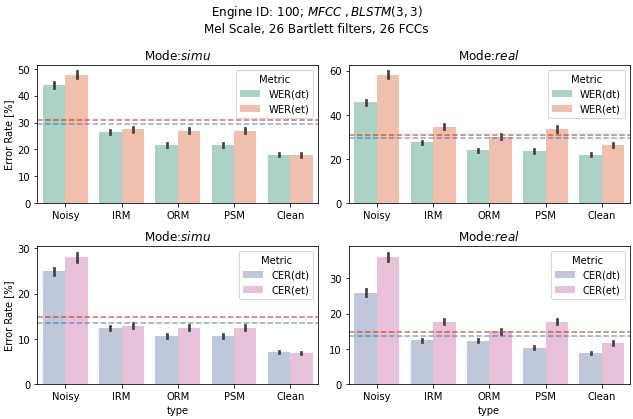
\includegraphics[width=0.95\linewidth]{ASR/images/asr100_wer_masks.png}
    \caption{ASR \#100 WER, CER vs. T-F masks, noisy and clean inputs }\label{fig:asr100_wer_masks}
\end{figure}

\subsubsection{ASR Engine \#101 --- Approx. Mel-FCC, \(\Delta,\Delta\Delta\), Context(3, 3)}
ASR Engine \#101 is identical to ASR engine \#100 except for the
actual implementation of the Mel scale. This engine has been
trained against the same features 
utilizing 
the linear approximation of the Mel scale
as described in Chapter\;\ref{ch:scaling_methods}.

\bigskip

Figures\;\ref{fig:asr_101},\;\ref{fig:asr101_wer}, 
and \ref{fig:asr101_wer_masks}
present the training, evaluation, and the 
T-F based beamforming results respectively. 

\begin{figure}[H]
    \centering
    \subfloat[\label{fig:asr_101}]{%
       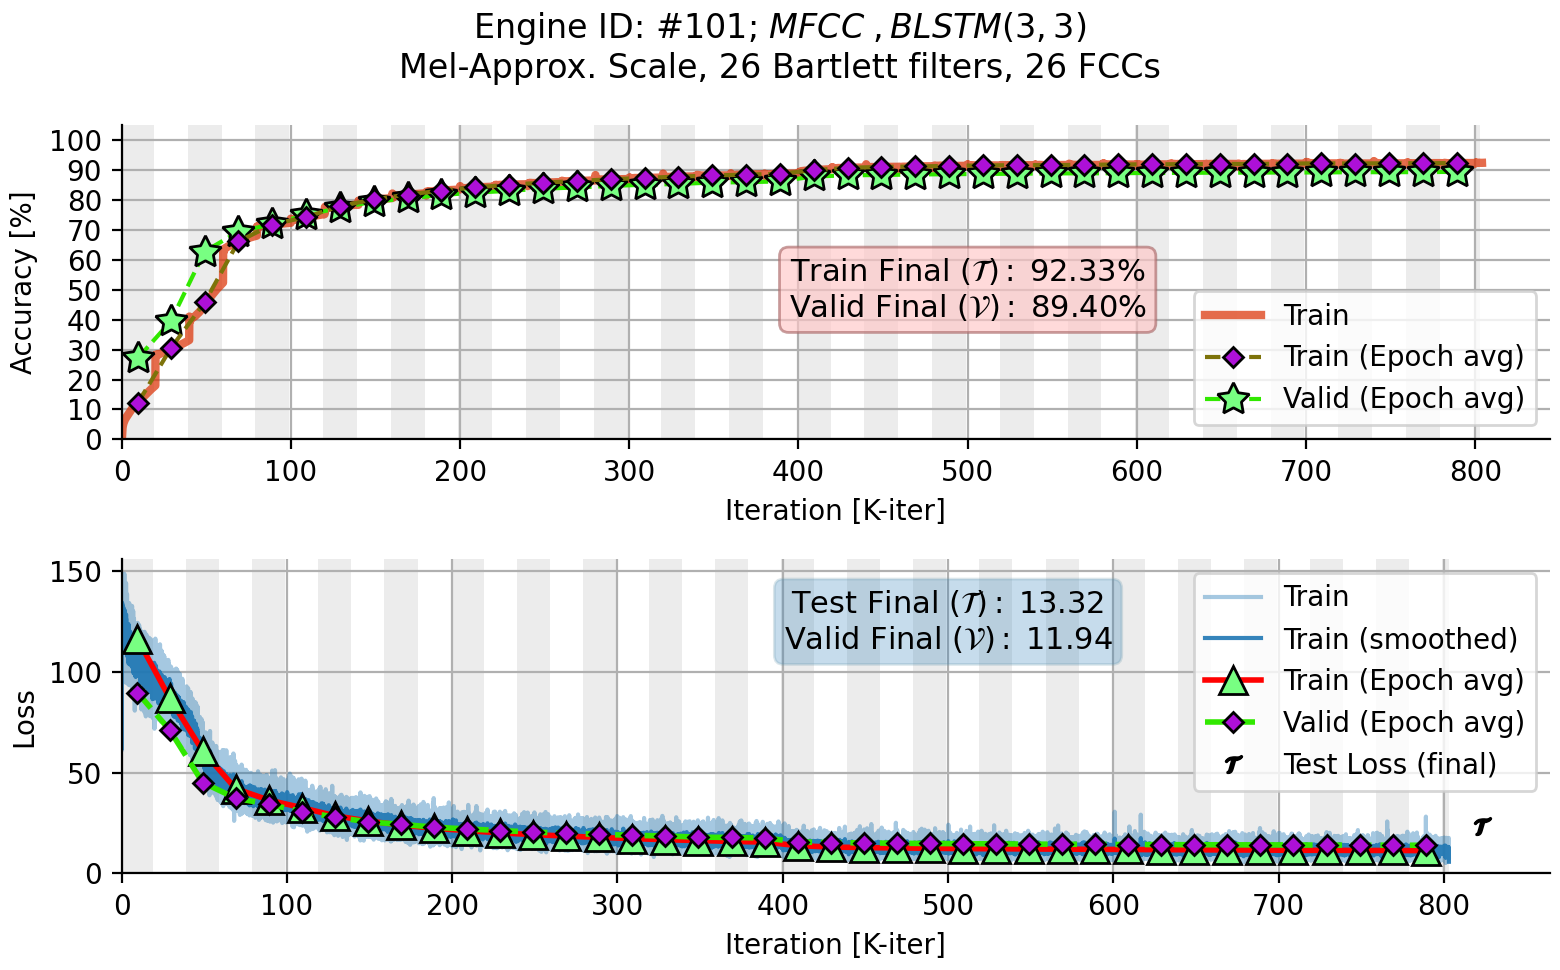
\includegraphics[width=0.85\linewidth]{ASR/images/asr_101}}
    \\
    \vspace{-0.3cm}
    \subfloat[\label{fig:asr101_wer}]{%
        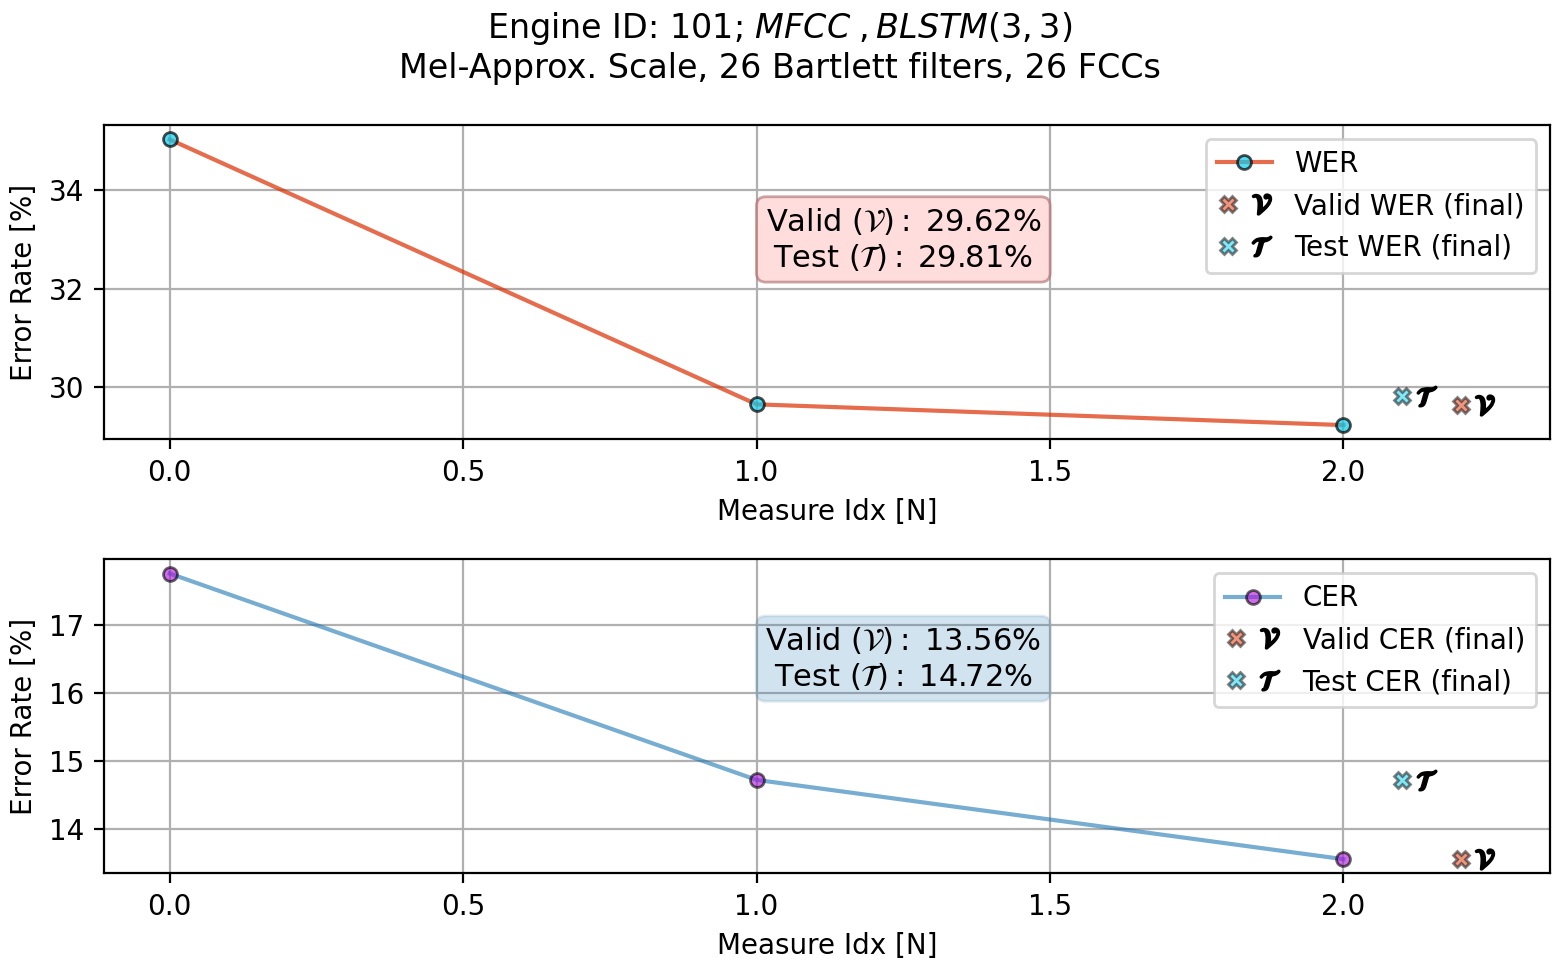
\includegraphics[width=0.85\linewidth]{ASR/images/asr101_wer.png}}
    \caption{(a) ASR \#12 training accuracy and loss plot;\;\;
        (b) ASR \#12 WER, CER evaluation plot.}\label{fig:asr101_wer_subplot} 
\end{figure}

\begin{figure}[H]
    \centering
    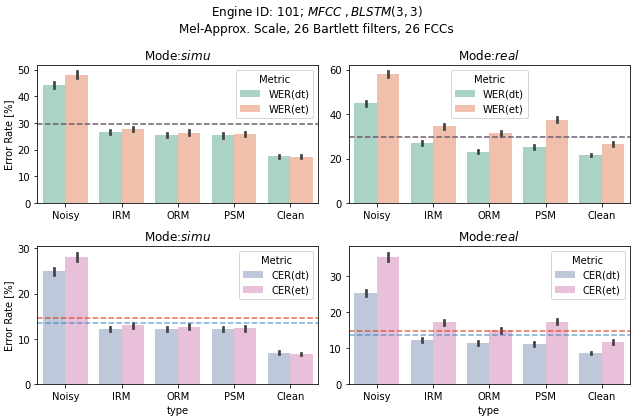
\includegraphics[width=0.95\linewidth]{ASR/images/asr101_wer_masks.png}
    \caption{ASR \#101 WER, CER vs. T-F masks, noisy and clean inputs }\label{fig:asr101_wer_masks}
\end{figure}


\subsubsection{Other ASR Engines}
ASR engines \#13, \#70, \#22, \#23
were not tested with the enhanced beamformed recordings.
The reason is that the performance of these ASR engines
is degraded compared to the previously described ASR engines.
However, for completeness, we present their training results
and some WER, CER measures for the training, validation,
and test subsets of the CommonVoice dataset.

\bigskip

Figures\;\ref{fig:asr_22},\;\ref{fig:wer_22}
present the training results and the WER and CER
metrics measures for ASR engine \#22.

\begin{figure}[H]
    \centering
    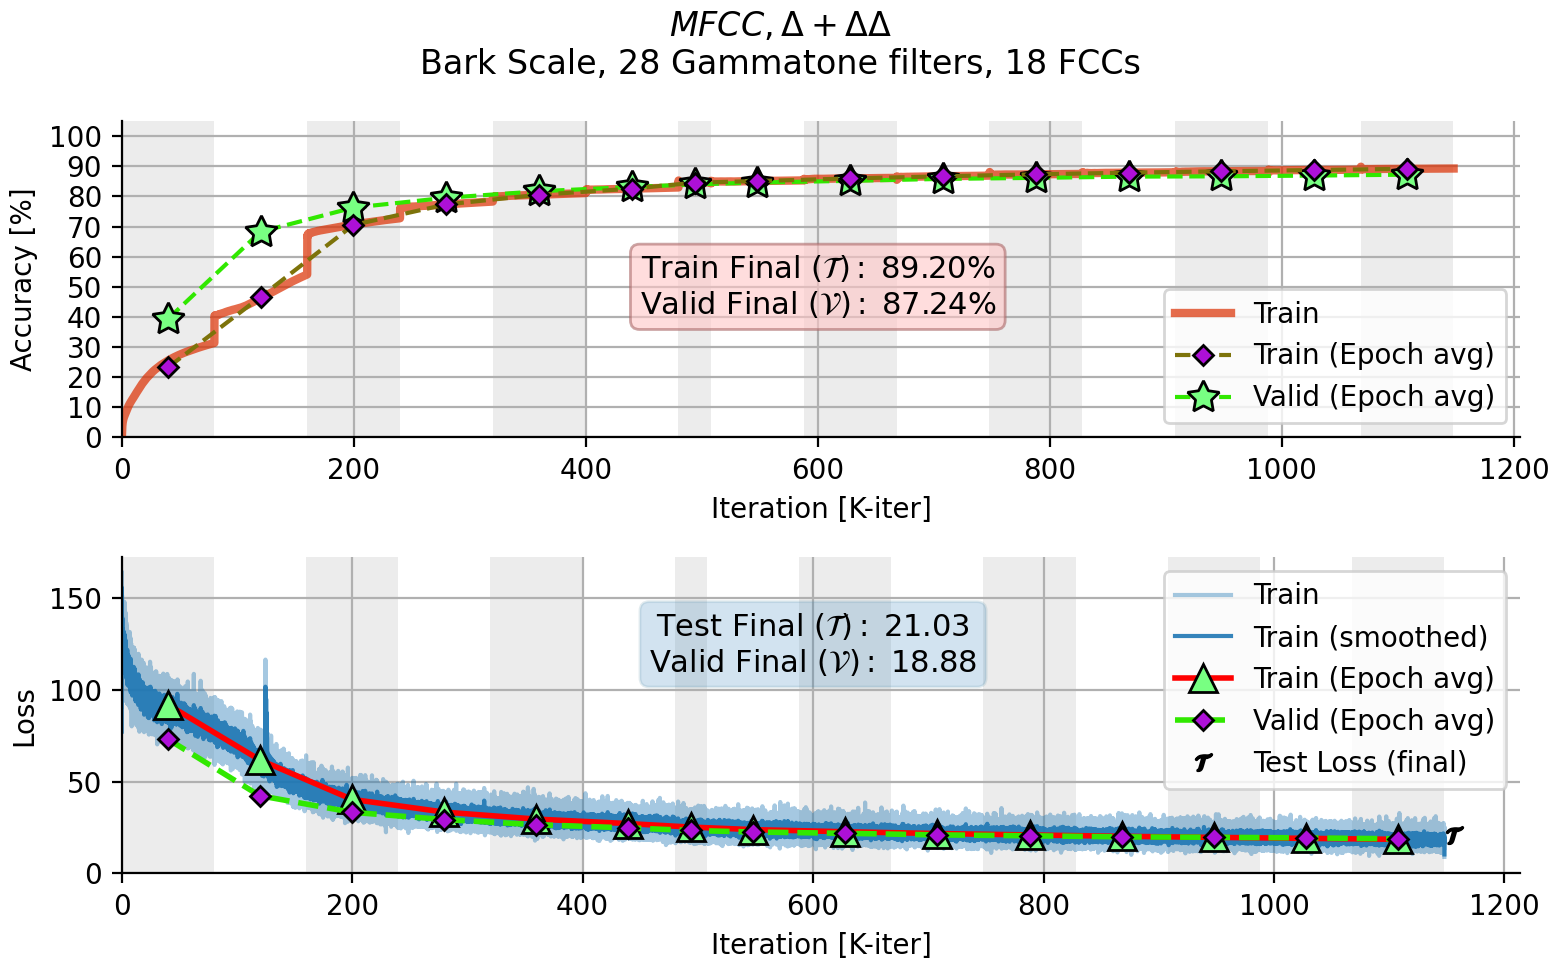
\includegraphics[width=0.95\linewidth]{Experiments/images/asr_22}
    \caption{ASR \#22 training accuracy and loss plot}\label{fig:asr_22}
\end{figure}

\begin{figure}[H]
    \centering
    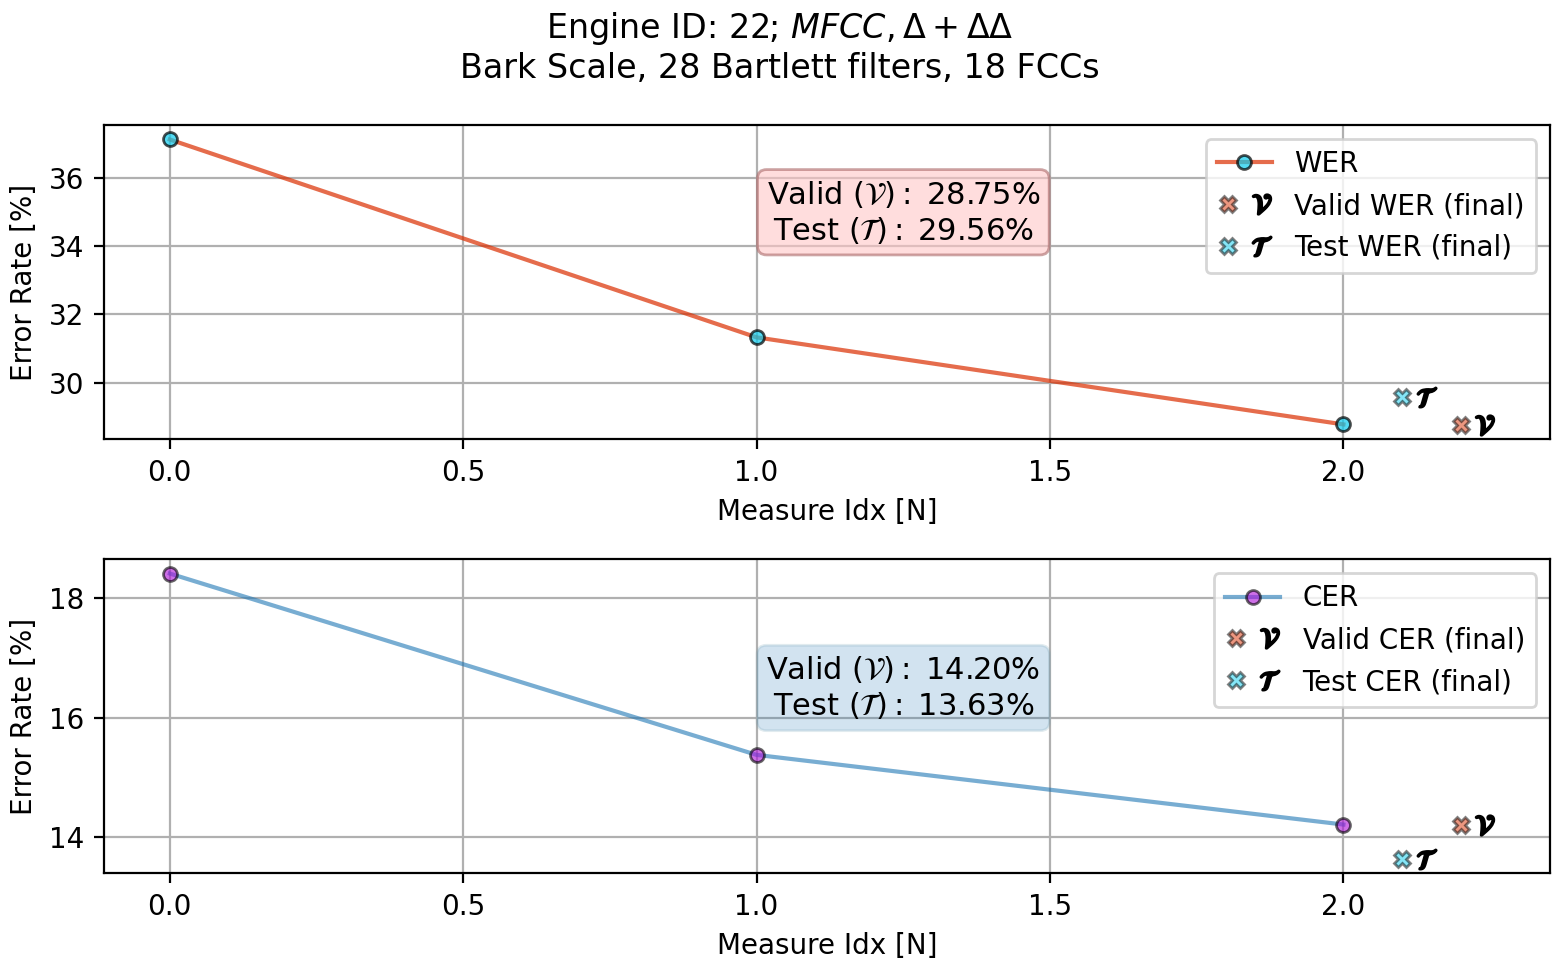
\includegraphics[width=0.95\linewidth]{ASR/images/asr22_wer.png}
    \caption{ASR \#22 WER, CER evaluation plot}\label{fig:wer_22}
\end{figure}

Figures\;\ref{fig:asr_23},\;\ref{fig:wer_23}
present the training results and the WER and CER
metrics measures for ASR engine \#23.

\begin{figure}[H]
    \centering
    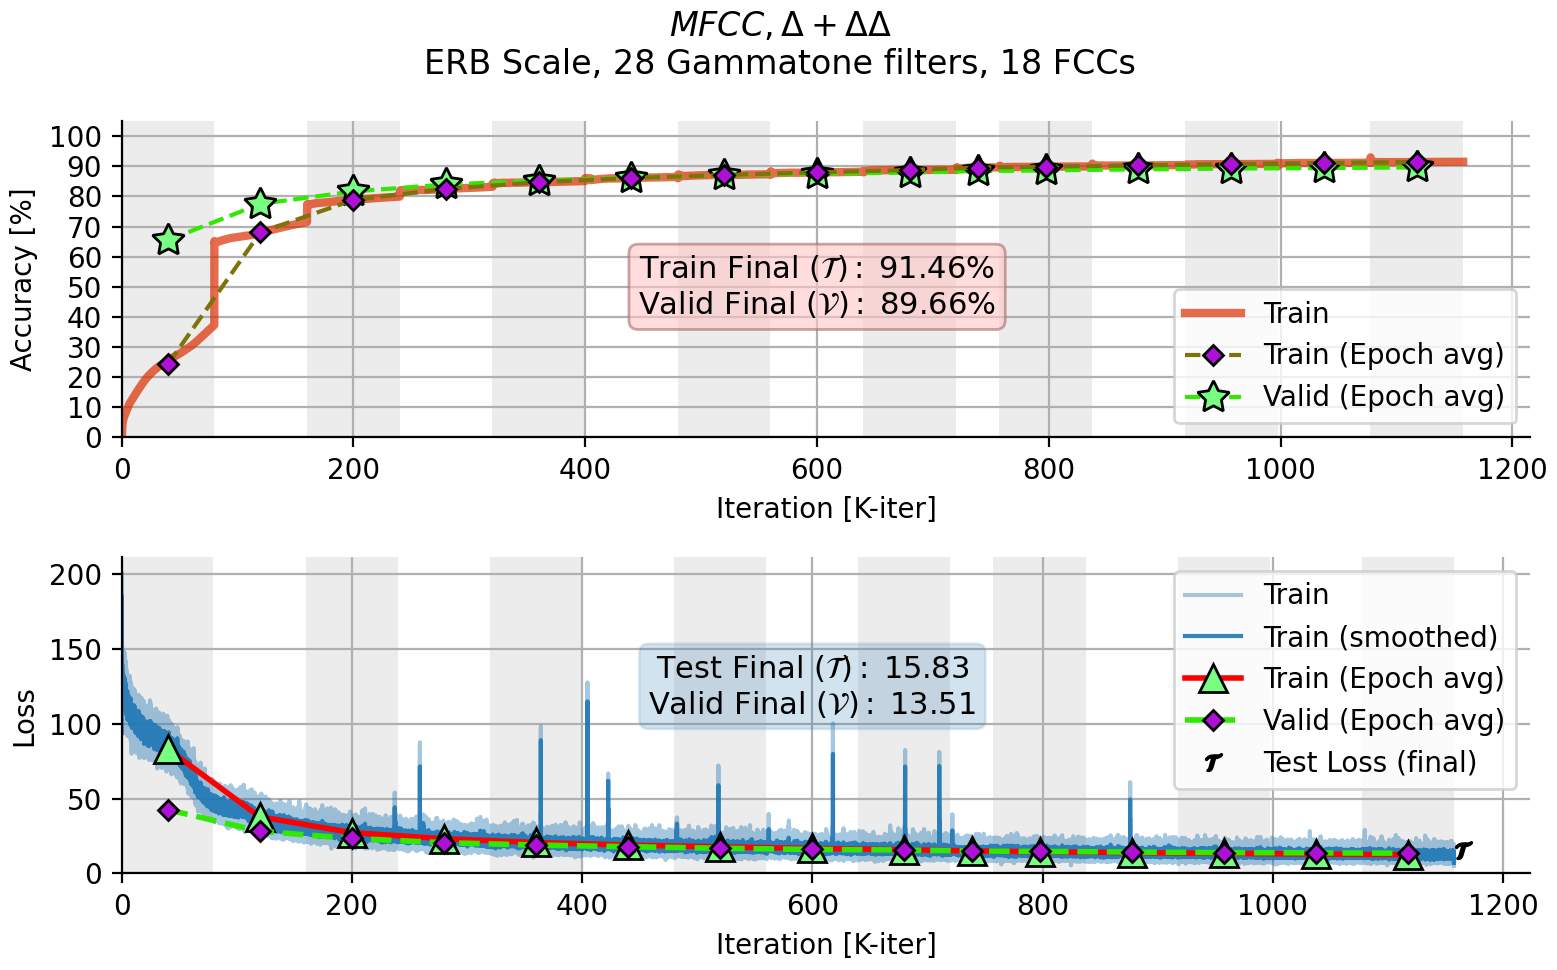
\includegraphics[width=0.95\linewidth]{Experiments/images/asr_23}
    \caption{ASR \#23 training accuracy and loss plot}\label{fig:asr_23}
\end{figure}

\begin{figure}[H]
    \centering
    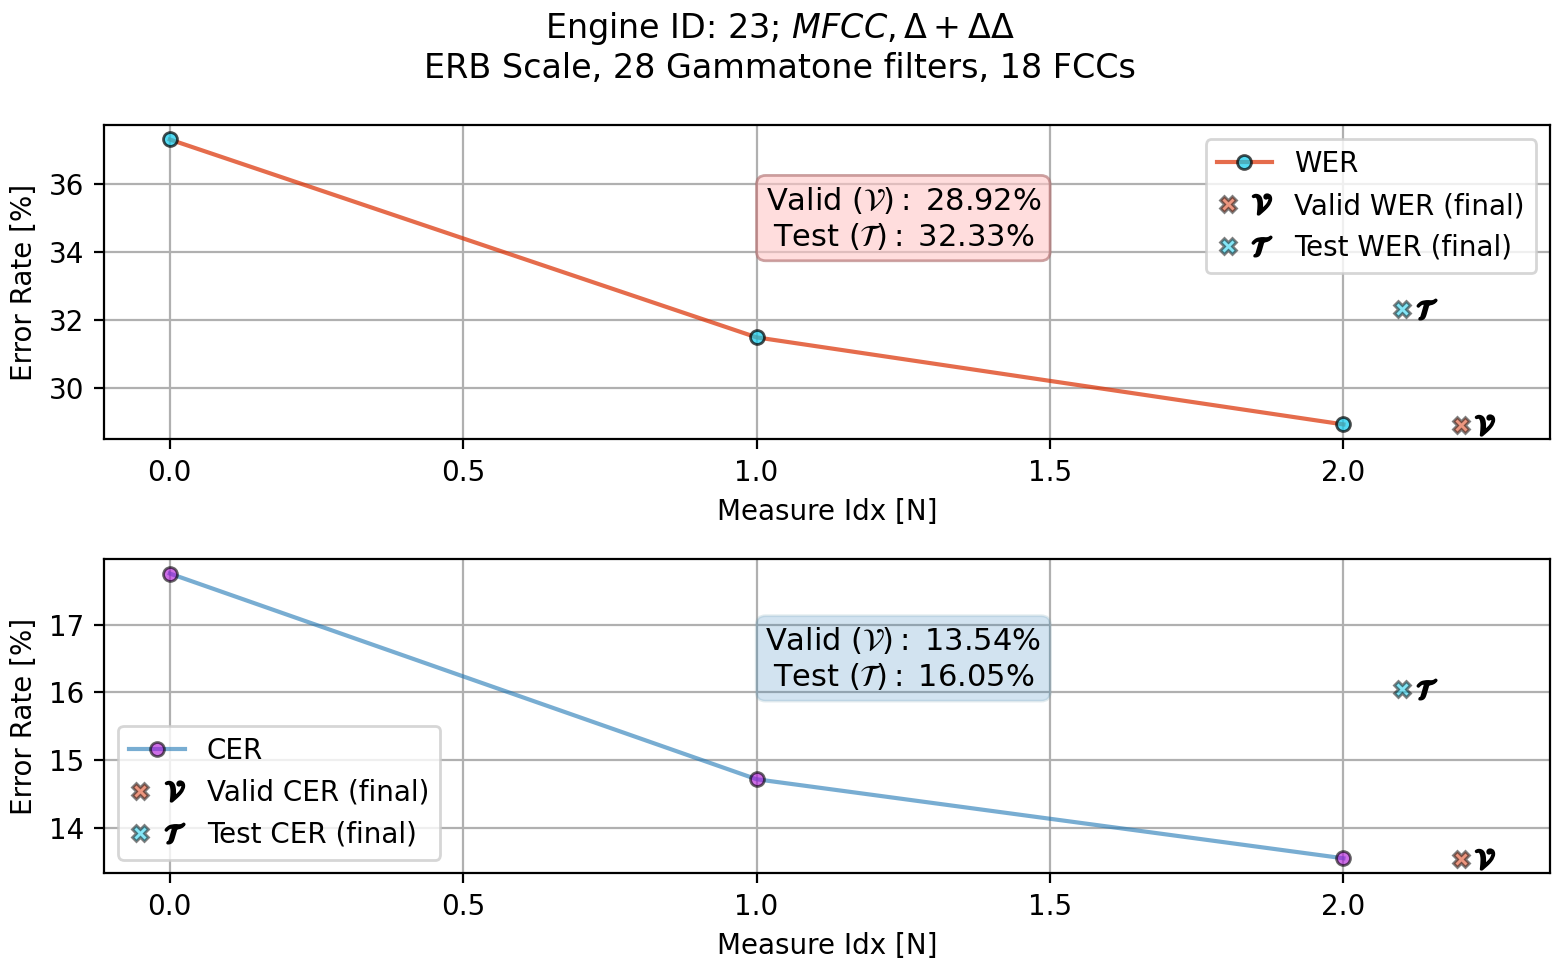
\includegraphics[width=0.95\linewidth]{ASR/images/asr23_wer.png}
    \caption{ASR \#23 WER, CER evaluation plot}\label{fig:wer_23}
\end{figure}

Figures\;\ref{fig:asr_70},\;\ref{fig:wer_70}
present the training results and the WER and CER
metrics measures for ASR engine \#70.

\begin{figure}[H]
    \centering
    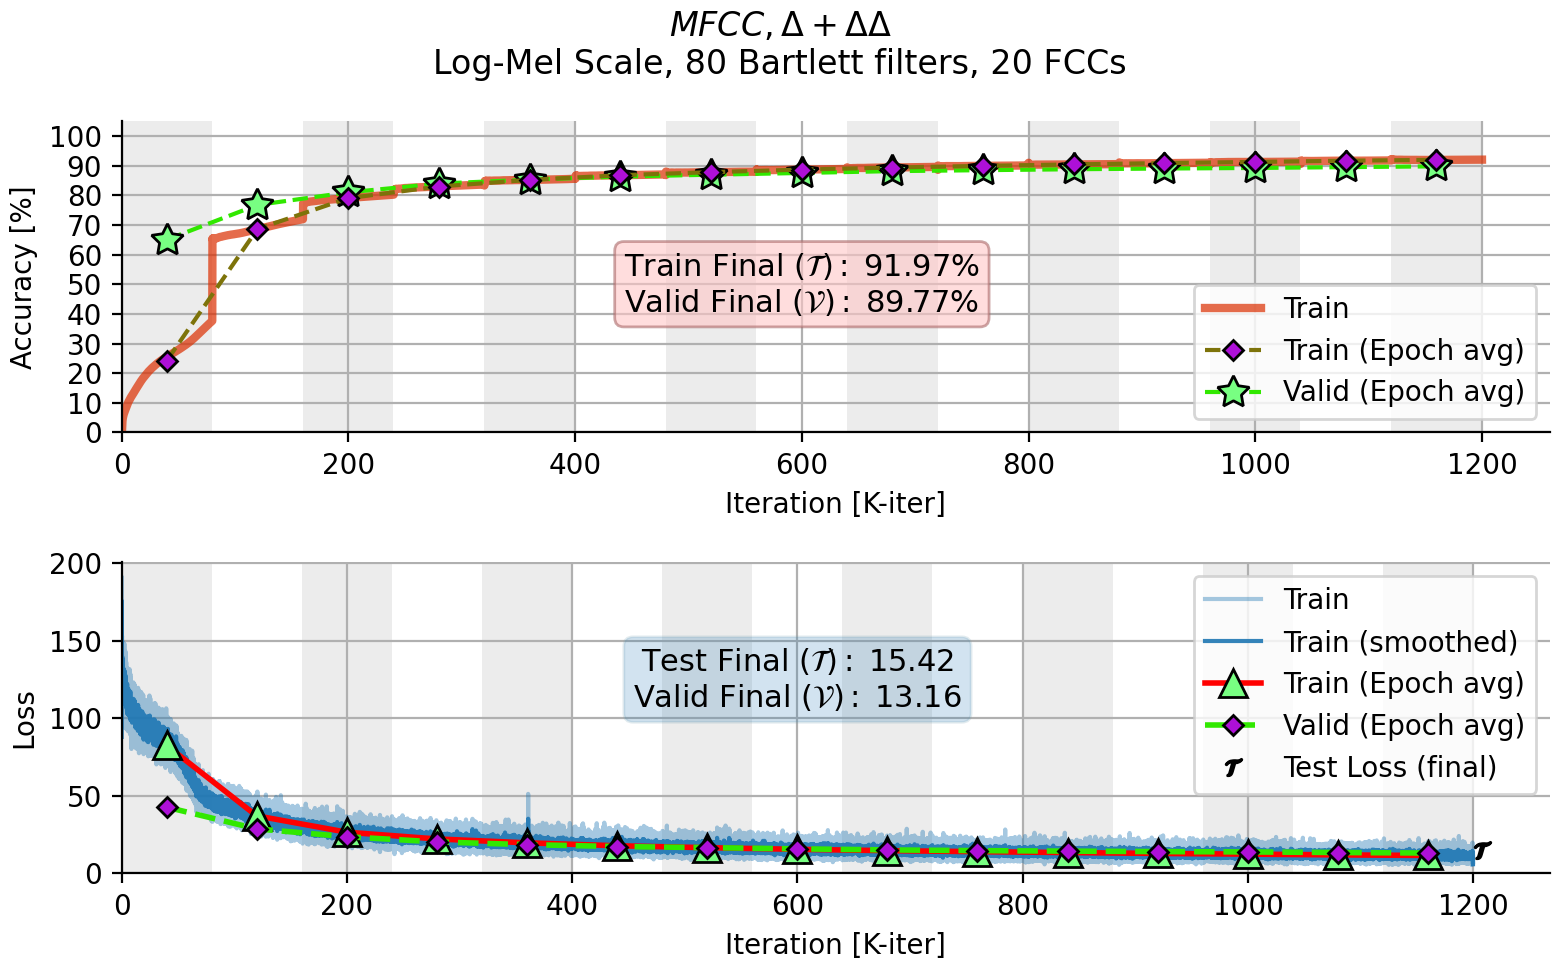
\includegraphics[width=0.95\linewidth]{Experiments/images/asr_70}
    \caption{ASR \#70 training accuracy and loss plot}\label{fig:asr_70}
\end{figure}

\begin{figure}[H]
    \centering
    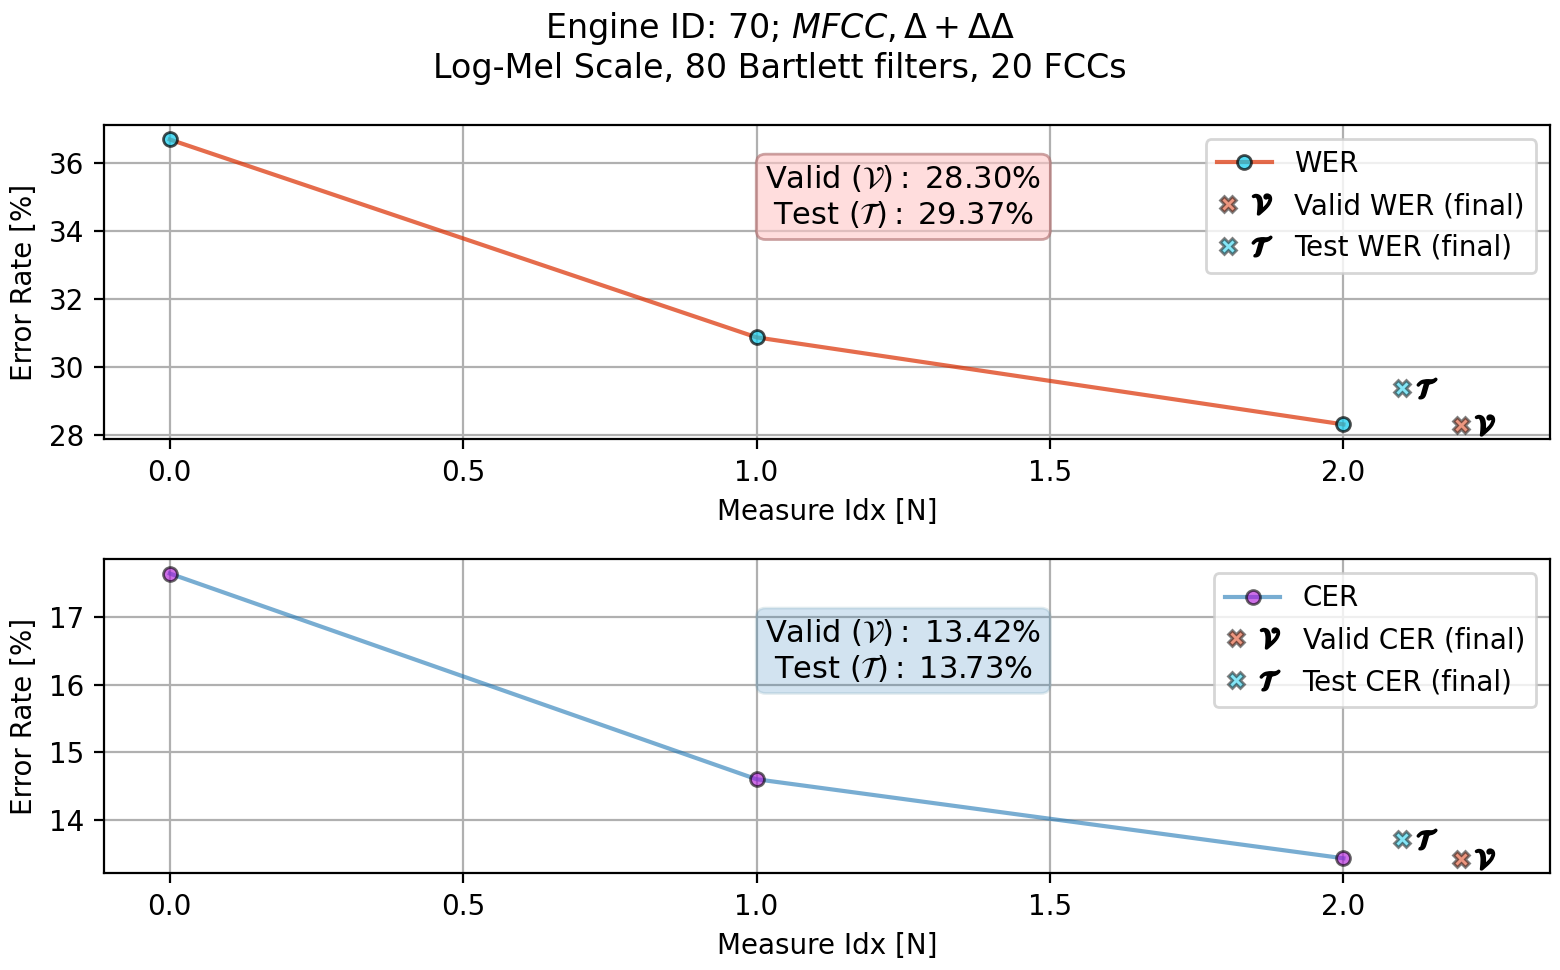
\includegraphics[width=0.95\linewidth]{ASR/images/asr70_wer.png}
    \caption{ASR \#70 WER, CER evaluation plot}\label{fig:wer_70}
\end{figure}

The training statistics were not gathered for ASR engine \#13,
so only the WER and CER measures for the validation
and test datasets are presented in Figure\;\ref{fig:wer_13}.

\begin{figure}[H]
    \centering
    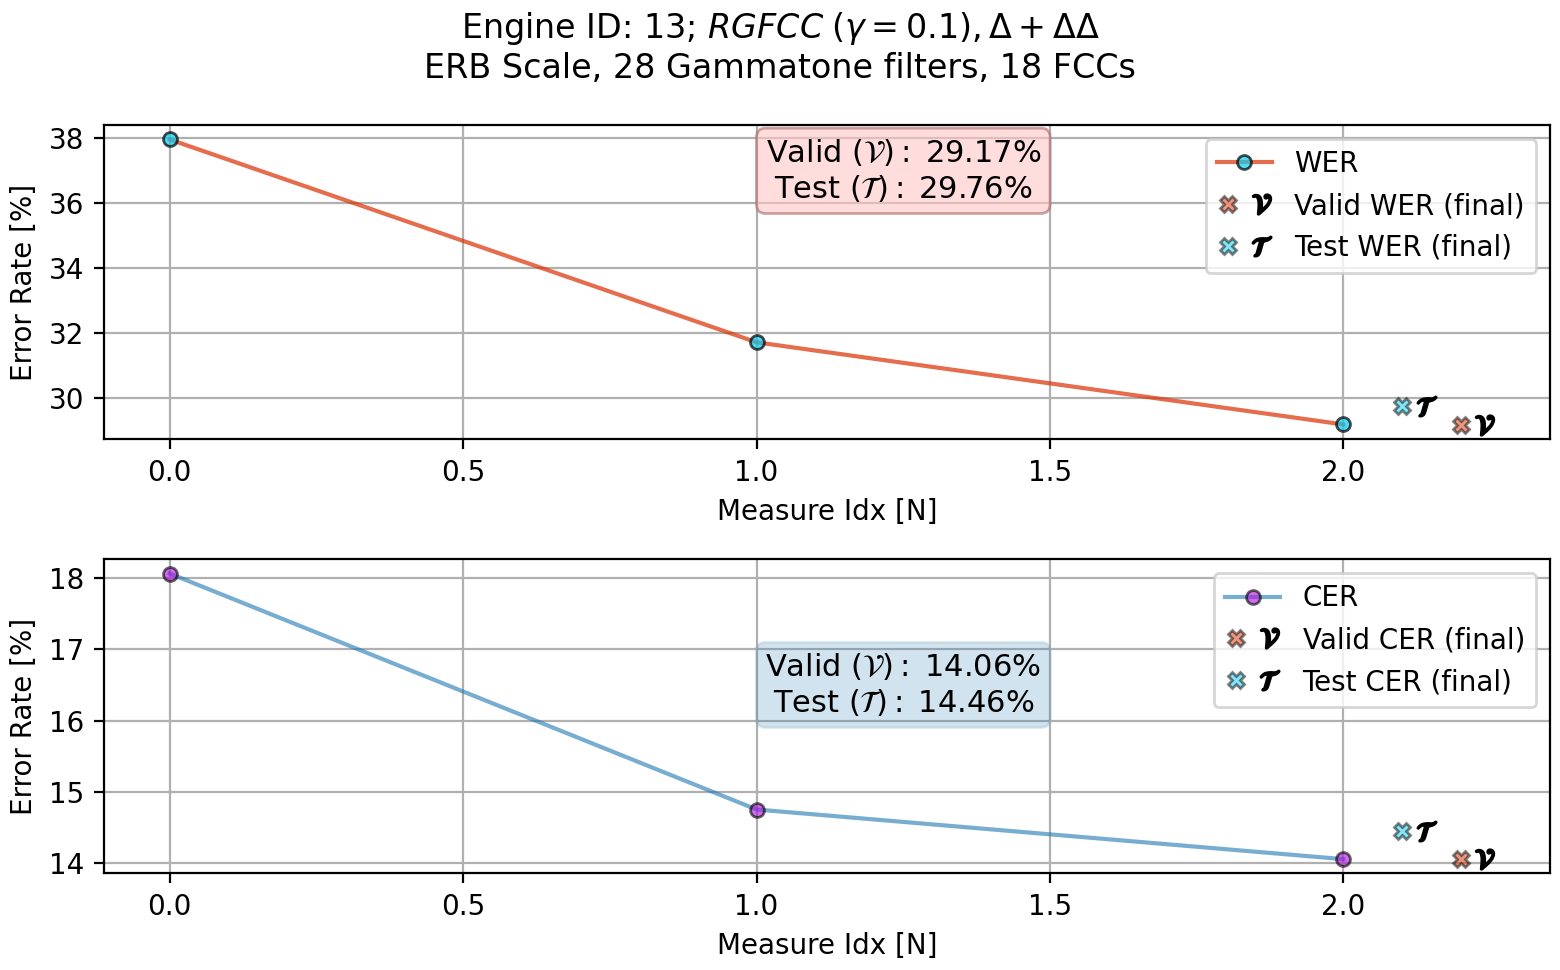
\includegraphics[width=0.95\linewidth]{ASR/images/asr13_wer.png}
    \caption{ASR \#13 WER, CER evaluation plot}\label{fig:wer_13}
\end{figure}


% \begin{figure}[H]
%     \centering
%     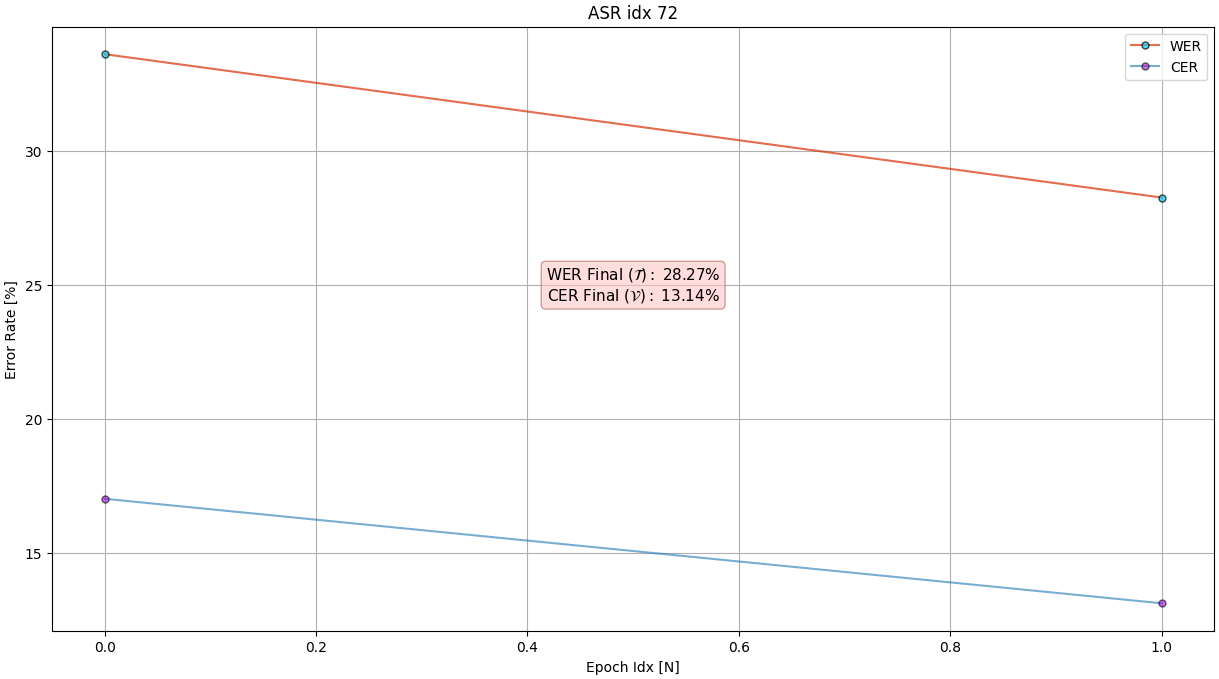
\includegraphics[width=0.75\linewidth]{Experiments/images/wer_72}
%     \caption{asr72}\label{fig:wer_72}
%     \end{figure}


% \begin{figure}[H]
%     \centering
%     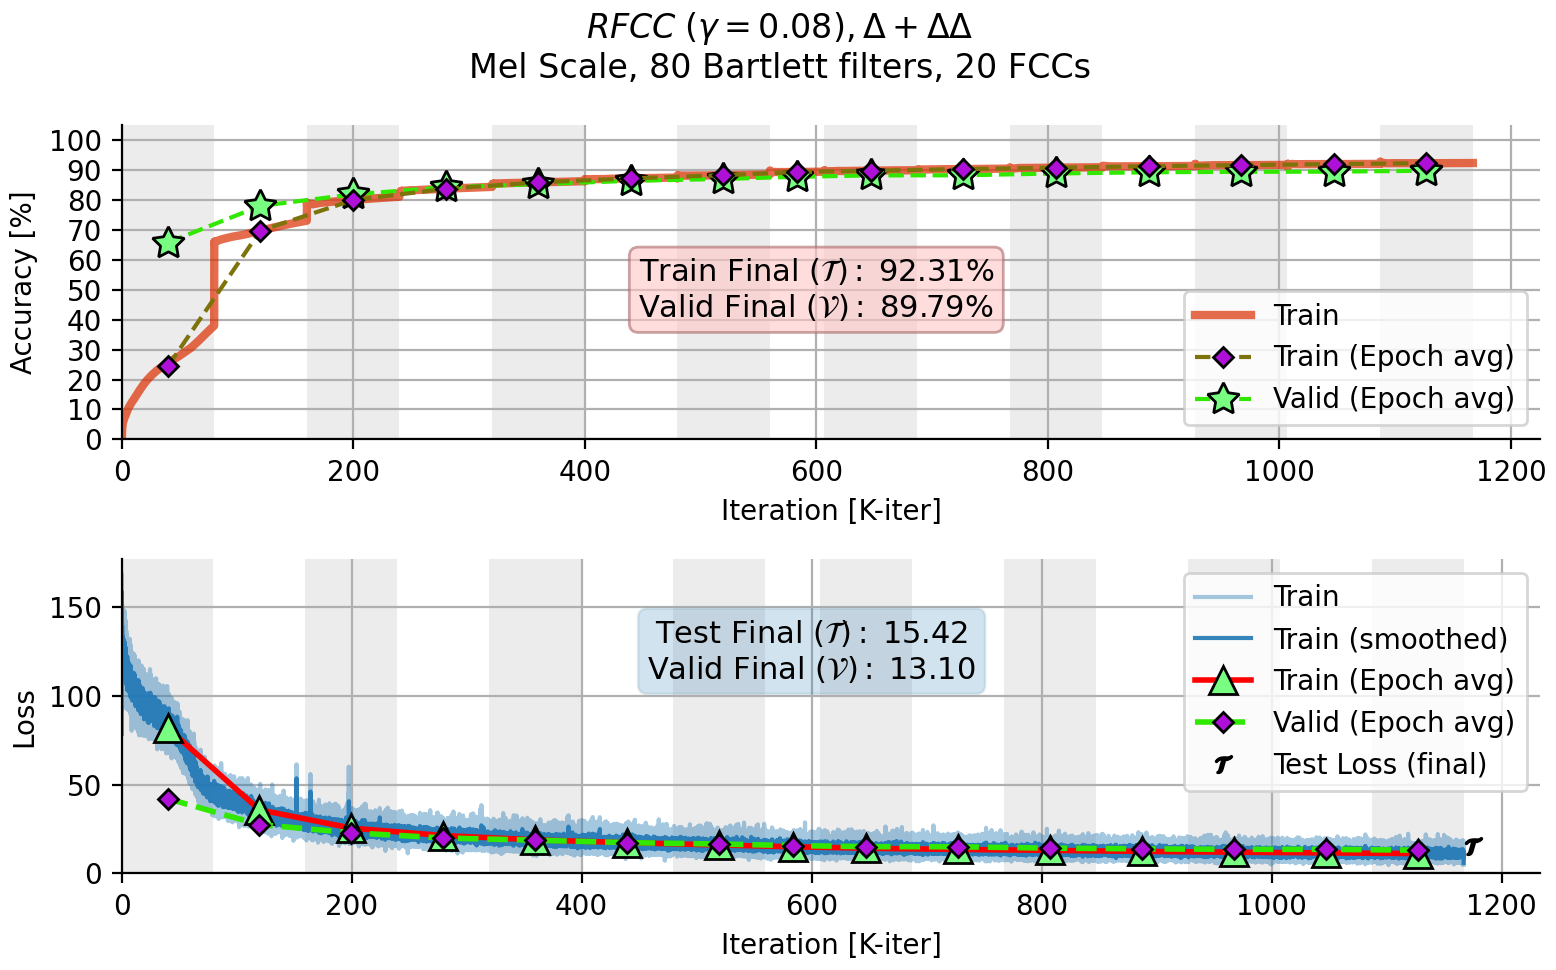
\includegraphics[width=0.75\linewidth]{Experiments/images/asr_15}
%     \caption{asr15}\label{fig:asr_15}
% \end{figure}

% \begin{figure}[H]
%     \centering
%     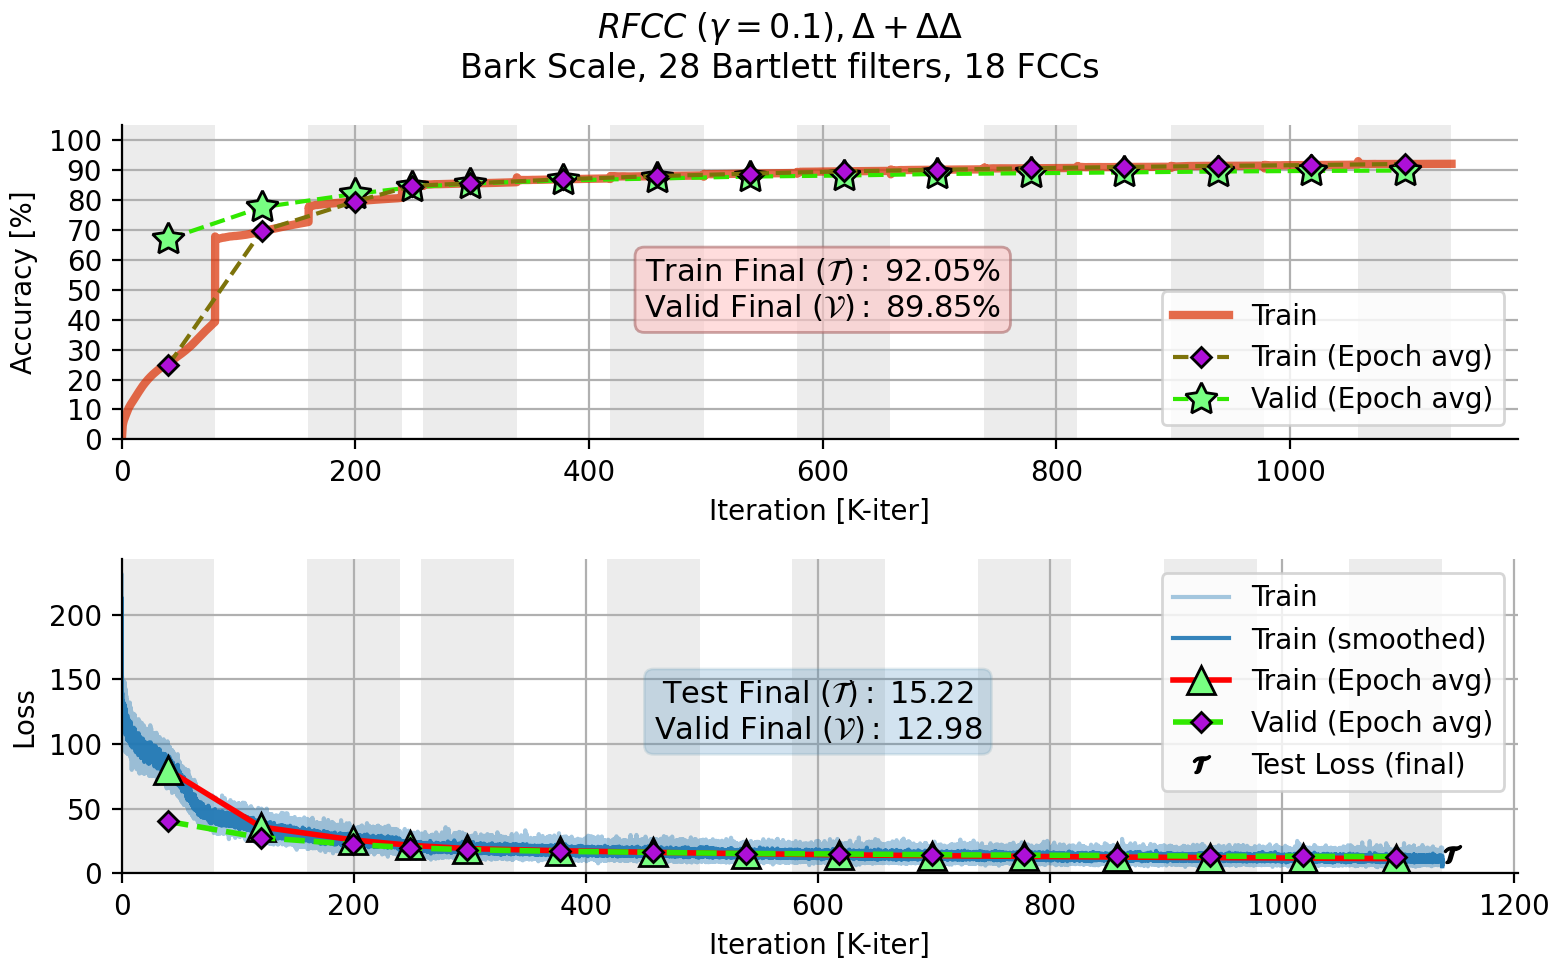
\includegraphics[width=0.75\linewidth]{Experiments/images/asr_12}
%     \caption{asr12}\label{fig:asr_12}
% \end{figure}

% \begin{figure}[H]
%     \centering
%     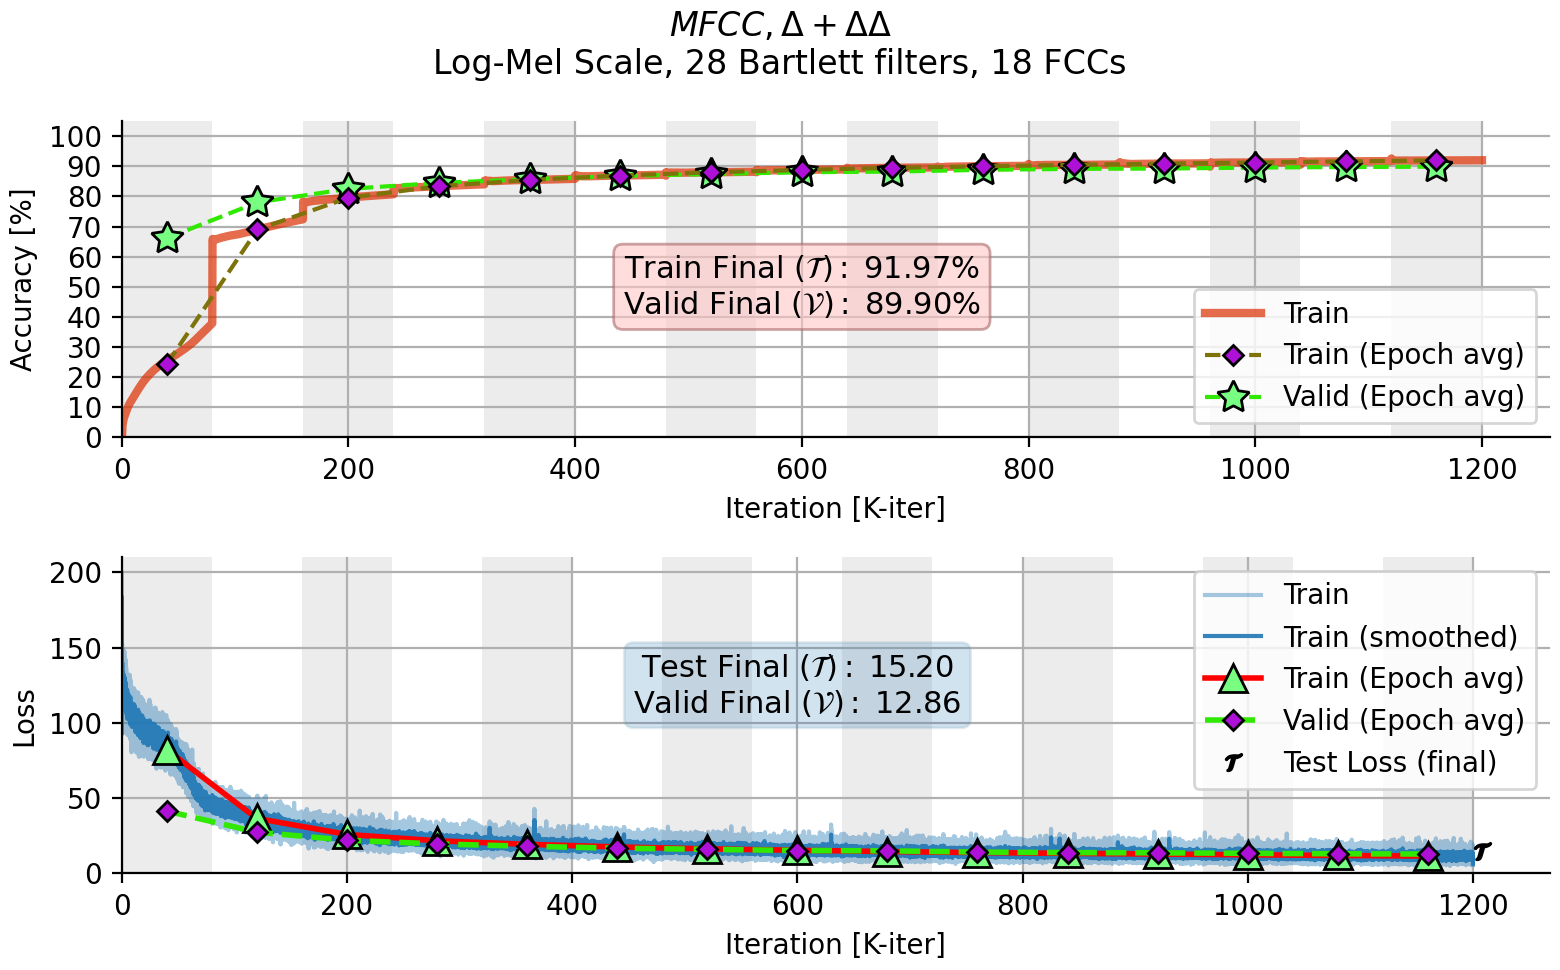
\includegraphics[width=0.75\linewidth]{Experiments/images/asr_72}
%     \caption{asr72}\label{fig:asr_12b}
% \end{figure}




% \begin{figure}[H]
% \centering
% 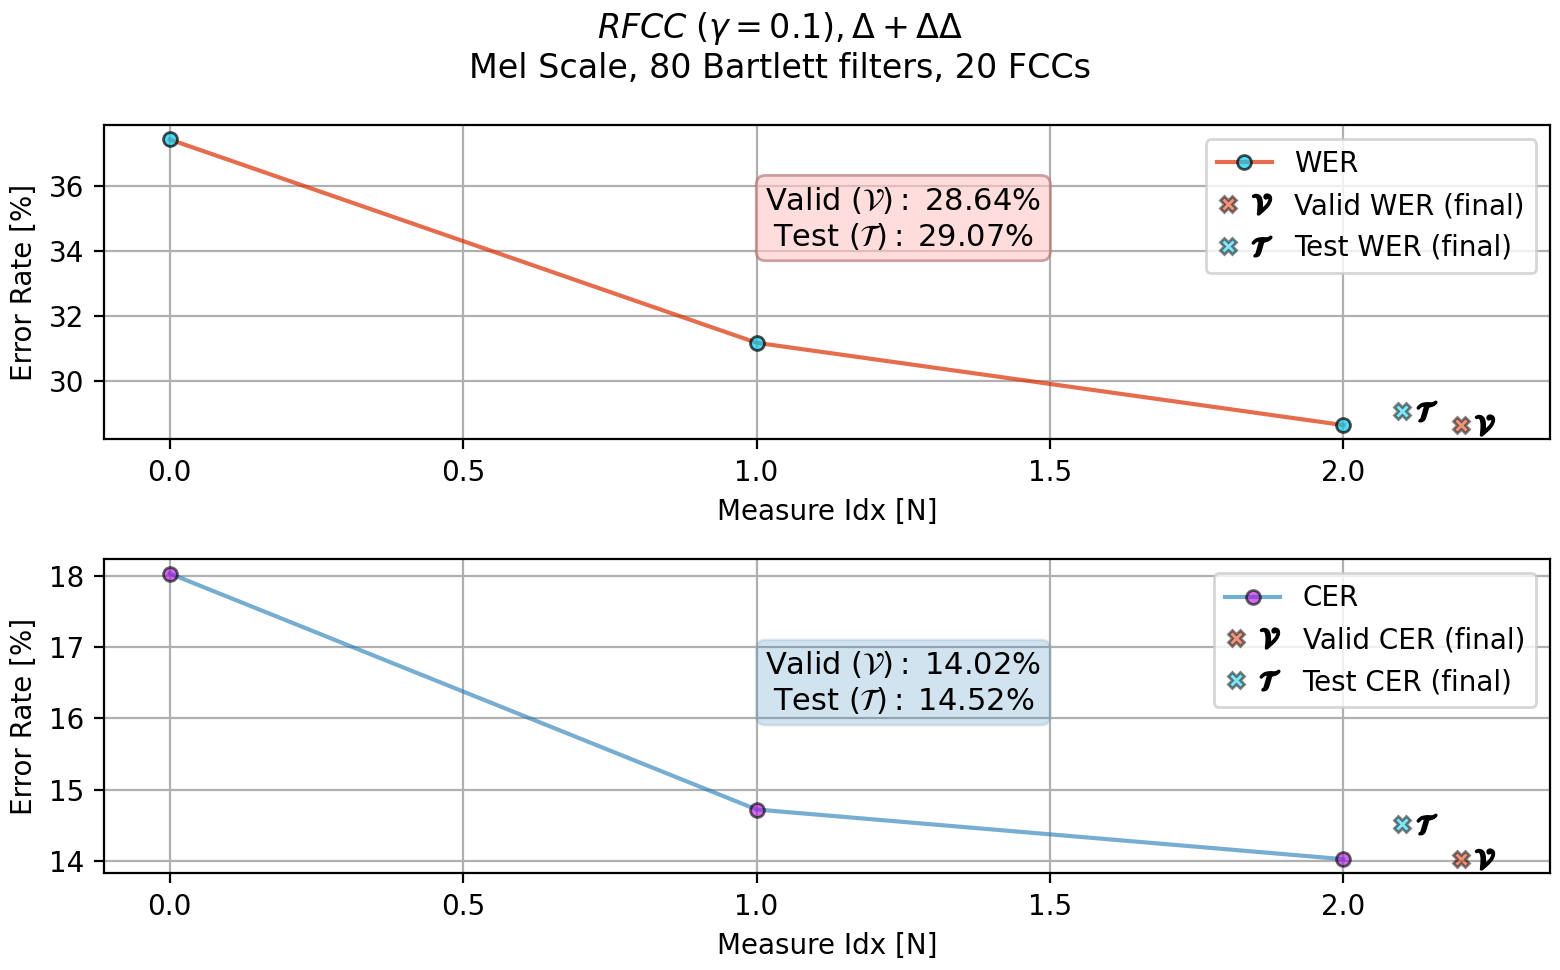
\includegraphics[width=0.75\linewidth]{Experiments/images/wer_5}
% \caption{asr5}\label{fig:wer_5}
% \end{figure}

% \begin{figure}[H]
% \centering
% 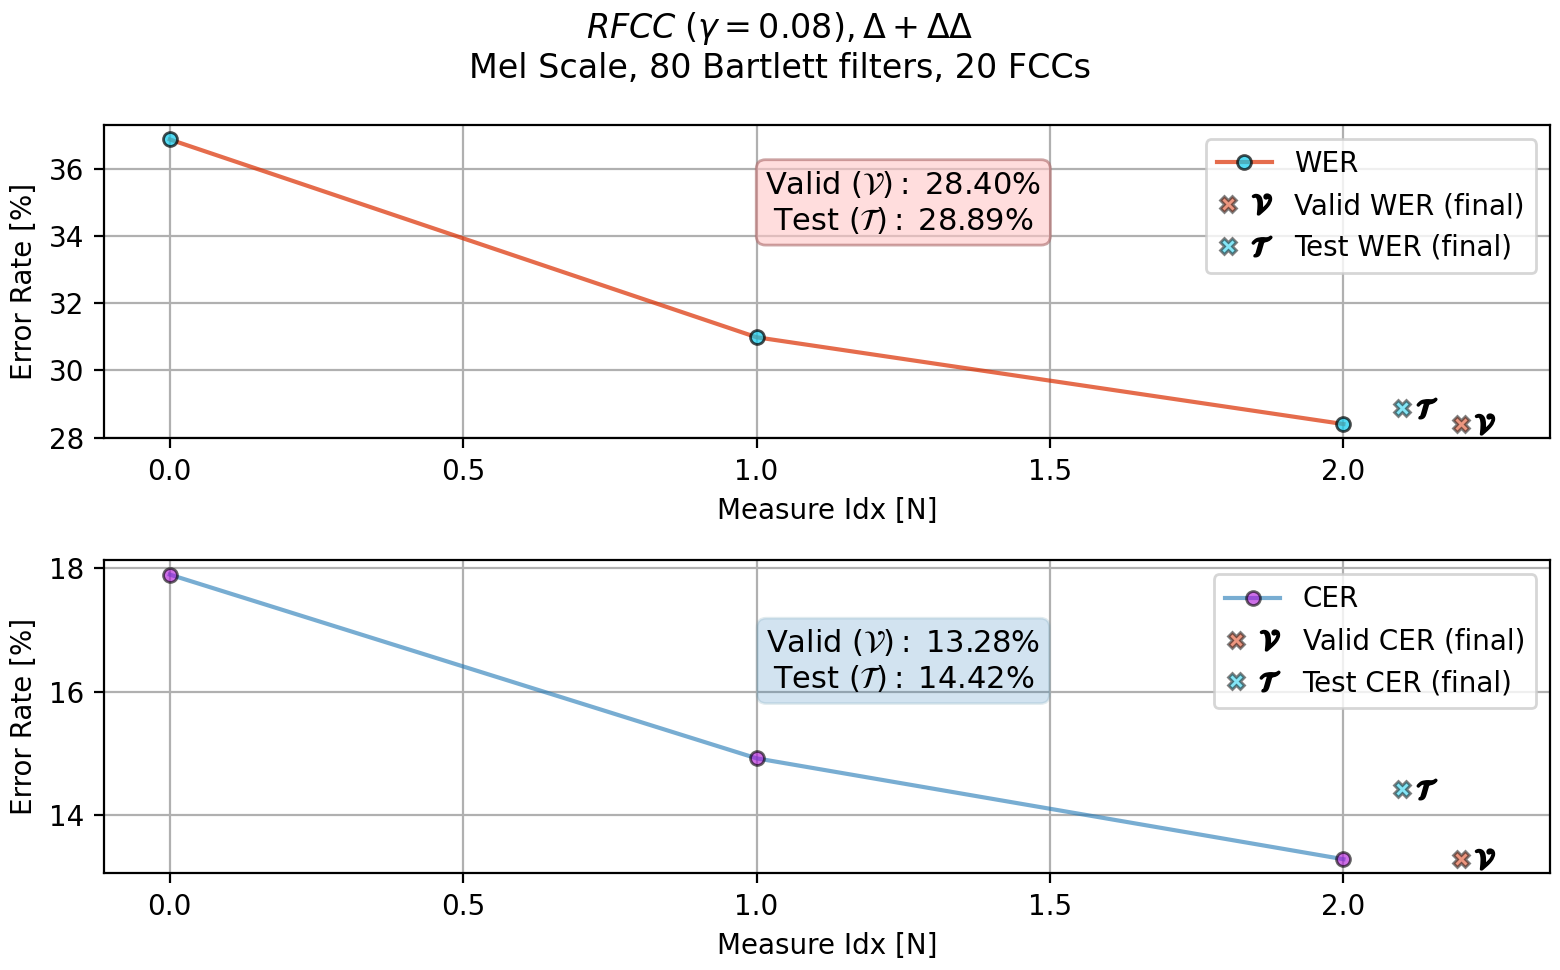
\includegraphics[width=0.75\linewidth]{Experiments/images/wer_15}
% \caption{asr15}\label{fig:wer_15}
% \end{figure}

% \begin{figure}[H]
% \centering
% 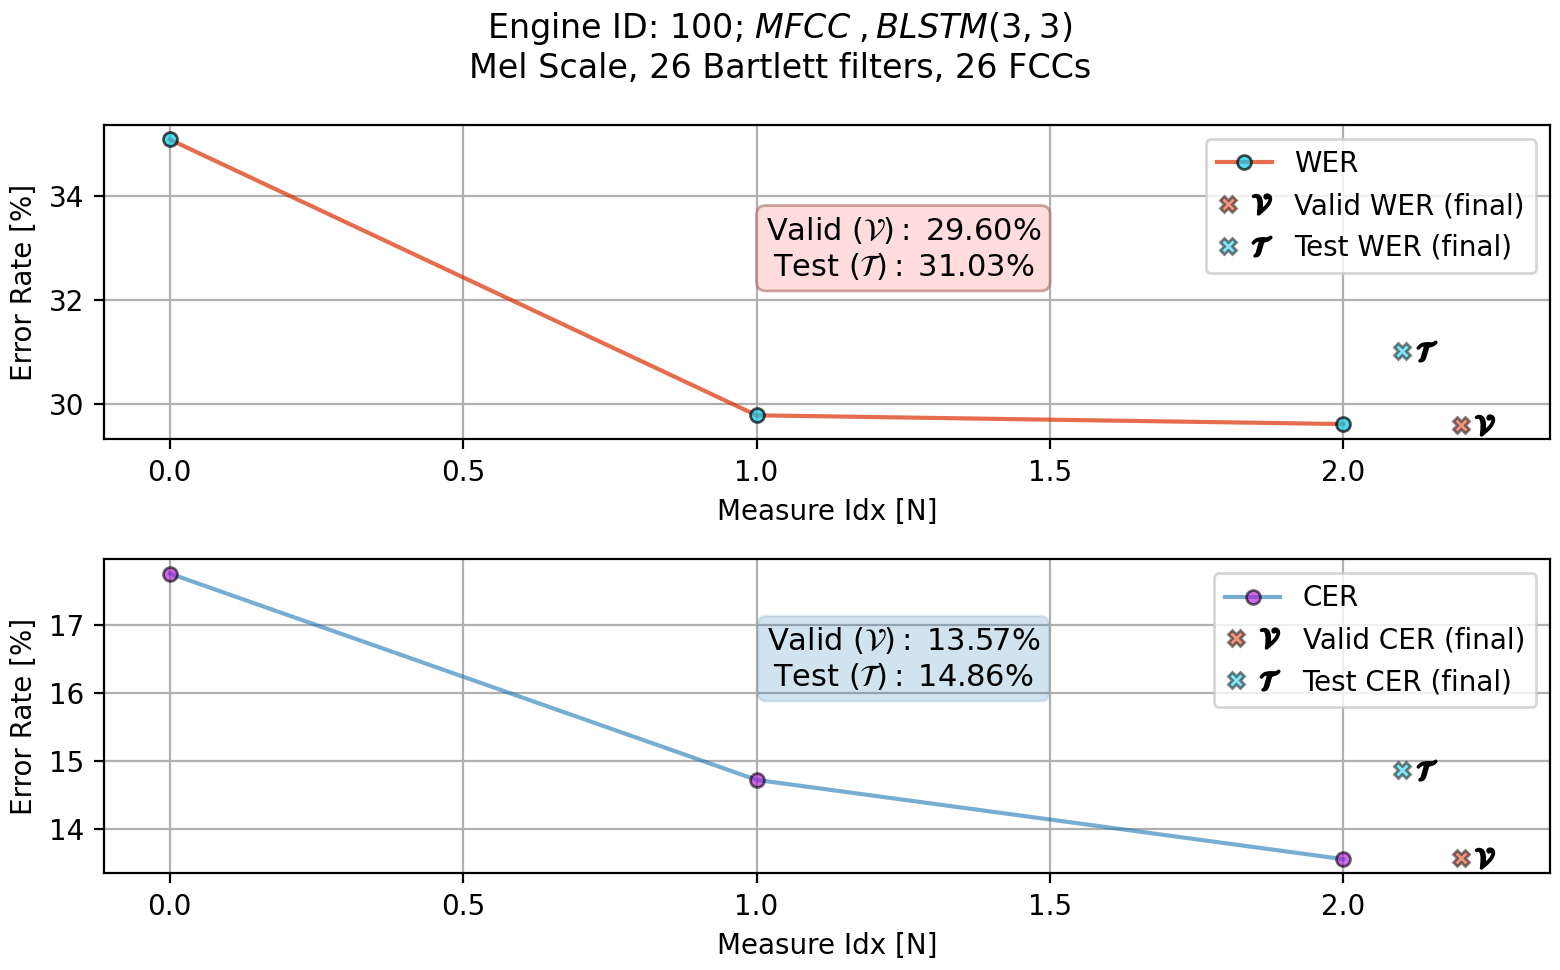
\includegraphics[width=0.95\linewidth]{ASR/images/asr100_wer}
% \caption{asr100}\label{fig:wer_100}
% \end{figure}

% \begin{figure}[H]
%     \centering
%     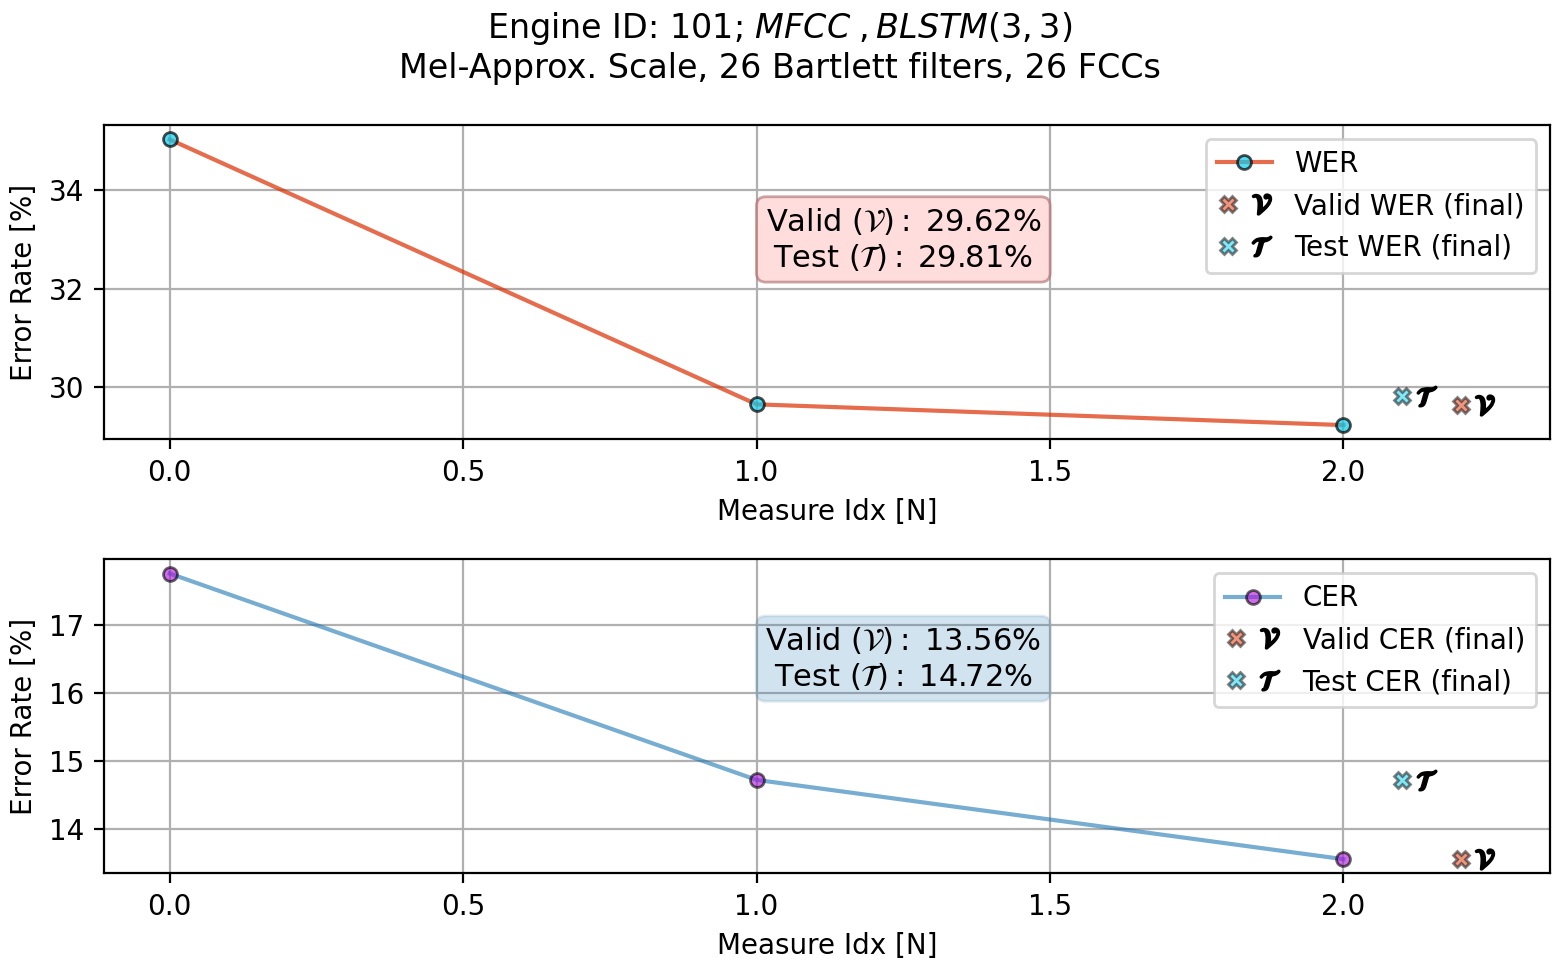
\includegraphics[width=0.95\linewidth]{ASR/images/asr101_wer}
%     \caption{asr101}\label{fig:wer_101}
% \end{figure}


    
% \begin{figure}[H]
% \centering
% 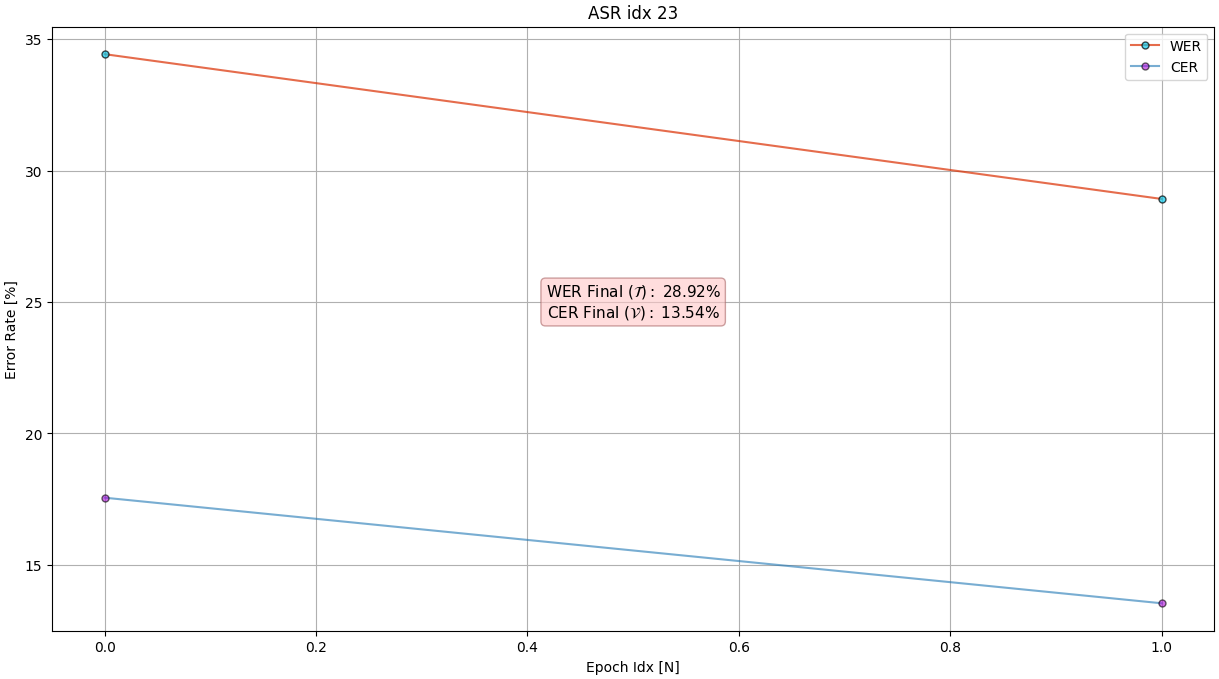
\includegraphics[width=0.95\linewidth]{Experiments/images/wer_23}
% \caption{asr23}\label{fig:wer_23}
% \end{figure}